\chapter{Analisi delle performance}

\label{Chapter4}

In questo capitolo interamente tecnico vengono presentati i risultati ottenuti in seguito alla valutazione di tre sistemi Linux differenti. Essendo tra le versioni più conosciute ed utilizzate al momento, si è deciso di effettuare il benchmark in Ubuntu, Debian e Mint in ambiente virtuale utilizzando come software per la creazione delle macchine VirtualBox. Si definisce il computer fisico \emph{host}, in quanto mette a disposizione il proprio spazio e l'hardware per virtualizzare il sistema definito \emph{guest} creato con VirtualBox.

Al fine di ottenere risultati confrontabili è necessario che durante la fase di testing non solo l'host rimanga nella medesimo stato per ogni guest, ovvero stessi programmi/processi in esecuzione, memoria, cpu disponibile ed altri valori, ma anche i guest devono eseguire il benchmark con le stesse risorse allocate.

Nella tabella sottostante vi sono le specifiche dei sistemi utilizzati:

\begin{table}[!htbp]
\label{tab:specs}
\centering
\begin{adjustbox}{width=\textwidth}
\begin{tabular}{|c|c|c|c|c|c|c|}
\hline
\textbf{Tipo} & \textbf{Modello} & \textbf{Sistema Operativo} & \textbf{Kernel} & \textbf{RAM(GB)} & \textbf{CPU} & \textbf{Core} \\
\hline
Host & MacbookPro (2015) & High Sierra v10.13.6 & Darwin v17.7.0 & 16 & IntelCore i7-4770HQ 2.2GHz & 4 \\
\hline
Guest & "" & Ubuntu v16.04.5 & Linux v4.15.0-29-generic &  2 & "" & 1 \\
\hline
Guest & "" & Debian v4.04.5 & Linux v4.9.0-7-amd64 &  2 & "" & 1 \\
\hline
Guest & "" & Mint v19 & Linux v4.15.0-20-generic &  2 & "" & 1 \\
\hline
\end{tabular}
\end{adjustbox}
\caption{Specifiche dei sistemi utilizzati}
\end{table}

Nonostante nella pagina di LKRG l'autore proponga gli esempi di rilevazione software solamente in ambiente Ubuntu v16.04, si è deciso di effettuare un'analisi anche nelle altre due distribuzioni, per poter osservare in che modo reagissero al caricamento del modulo e soprattutto se nella stessa maniera, oppure con qualche differenza. Dovendo testare system call comuni a tutte le distribuzioni Linux, non vi è alcun problema di compatibilità nell'utilizzo di SysBench nei tre guest.

In alcune verifiche effettuate è risultata una netta differenza di tempi d'esecuzione delle funzioni con LKRG attivo e non, per cui volendo confrontare dei dati così diversi si è scelto di utilizzare una scala logaritmica per l'asse delle ordinate (y) o delle ascisse (x) a seconda della tipologia di grafico. È importante sottolineare questo dettaglio, perchè la lettura del grafico è leggermente differente: mentre solitamente osservando l'asse y notiamo un aumento caratterizzato da step lineari (esempio: 1, 2, 3, ..., 10), utilizzando la scala logaritmica la distribuzione dei valori è differente, in quanto la distanza tra i punti è calcolata utilizzando il logaritmo secondo la legge $\lambda (OA)= \log (a)$ che rappresenta a distanza tra un punto di coordinata (0, a) e l'origine dell'asse y O è data da .

Prendiamo come esempio la scala logaritmica in base 10 utilizzata in questo elaborato osservando la figura sottostante in cui vi sono riportate alcune potenze:

\begin{figure}[!ht]
\centering
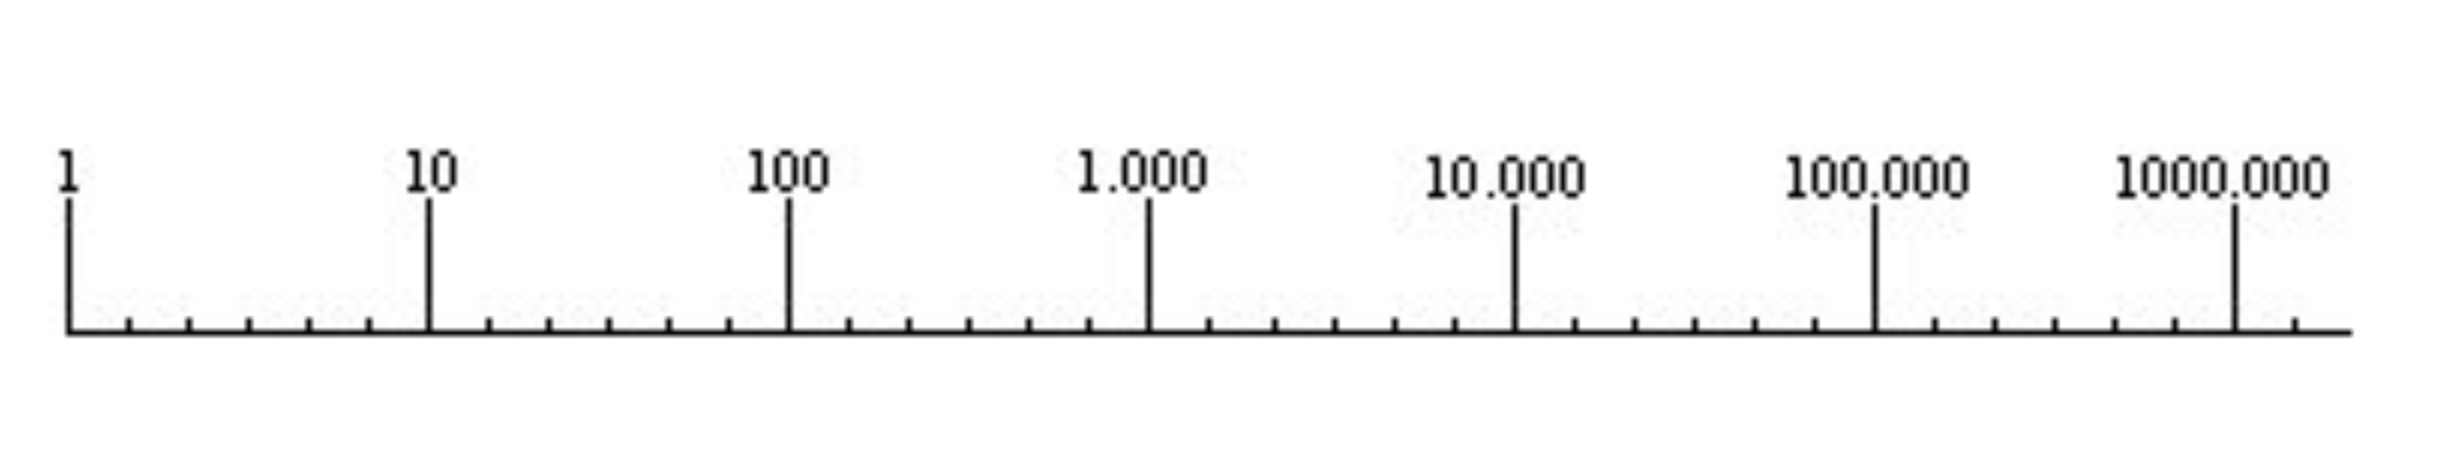
\includegraphics[scale=0.2]{Figures/LogarithmicScale}
\caption[Scala logaritmica di base 10.]{Scala logaritmica di base 10.\\Fonte: \href{https://it.wikipedia.org/wiki/Scala_logaritmica}{https://en.wikipedia.org}}
\label{fig:logarithmicScale}
\end{figure}

Il valore \emph{1} è calcolabile come la distanza tra il punto d'origine O e sé stesso, ovvero: $\lambda (OO) = 0 => \log (x_0) = 0 => x_0 = 1$. Ugualmente il valore \emph{10} che rappresenta il primo step è dato da $\lambda (OA) = 1 => \log (x_1) = 1 => x_1 = 10$.

Essendo abituati alla scala lineare, verrebbe da pensare che il punto medio tra l'1 ed il 10 di distanza 0.5 dall'origine rappresenti il valore 5; in realtà nella scala logaritmica applicando il calcolo si ottiene $\lambda (OM) = 0.5 => \log (x_m) = 0.5 => x_m = 1/\sqrt{10} \approx 3.16$.

In questa maniera è vero che si perde un po' di precisione del dato, ma è possibile raffigurare valori estremamente differenti, persino con ordini di grandezza doppi o tripli.

Al fine di una buona lettura, si ricorda che in ogni grafico sono riportati i parametri \emph{ncycle} ed \emph{nproc}, i quali corrispondono al numero di singole system call invocate e processi creati (esempio: ncycle=100 significa che la system call X è stata eseguita 100 volte). Inoltre nei grafici sono stati utilizzati i simboli matematici per indicare:

\begin{itemize}
\item \bm{$\sigma$}: la deviazione standard, ovvero l'indice di dispersione dei dati rispetto la media aritmetica;
\item \bm{$\overline{x}}$: per indicare il tempo di esecuzione medio della singola system call, calcolato dividendo i tempi ottenuti per il numero di system call invocate.
\end{itemize}

Infine, i risultati presentati sono stati ricavati mediante diversi test, in alcuni dei quali certe system call hanno un tempo d'esecuzione pari a 0. Per coerenza si è deciso di non rimuovere tali informazioni nei grafici, nonostante possa sembrare leggermente più complessa la lettura dei valore lungo l'asse delle y. Pertanto quando lungo tale asse è indicato il valore $0.00e^{+0}$, si prenda come riferimento per i valori leggermente superiori l'ordine di grandezza $1.00e^{-7}$, il secondo valore più piccolo misurato.

%----------------------------------------------------------------------------------------
%	UBUNTU TESTS
%----------------------------------------------------------------------------------------
\section{Test in Ubuntu}

L'analisi di LKRG in Ubuntu ha presentato risultati interessanti, soprattutto confrontando le diverse modalità d'esecuzione del programma. Iniziamo osservando il grafico sottostante, ottenuto eseguendo lo script mediante il quale avvengono 50 esecuzioni consecutive di SysBench con ncycle=1 (e non una singola esecuzione con ncycle=50 che verrà discussa in seguito), salvando i risultati in altrettanti file di output. In questo modo non vi possono essere ottimizzazioni dovuti alla cache, in quanto essendo una memoria veloce e piccola in cui vengono memorizzati i dati recentemente usati dalla memoria principale (RAM), ogni volta che la system call viene invocata il sistema salva le informazioni relative a tale funzione nella cache, ma non ne farà uso per il semplice motivo che il programma richiama la funzione una singola volta, mentre come vedremo in seguito tale memoria incide sul tempo d'esecuzione nel caso la stessa esecuzione richiami la system call più volte.

\begin{figure}[!ht]
\centering
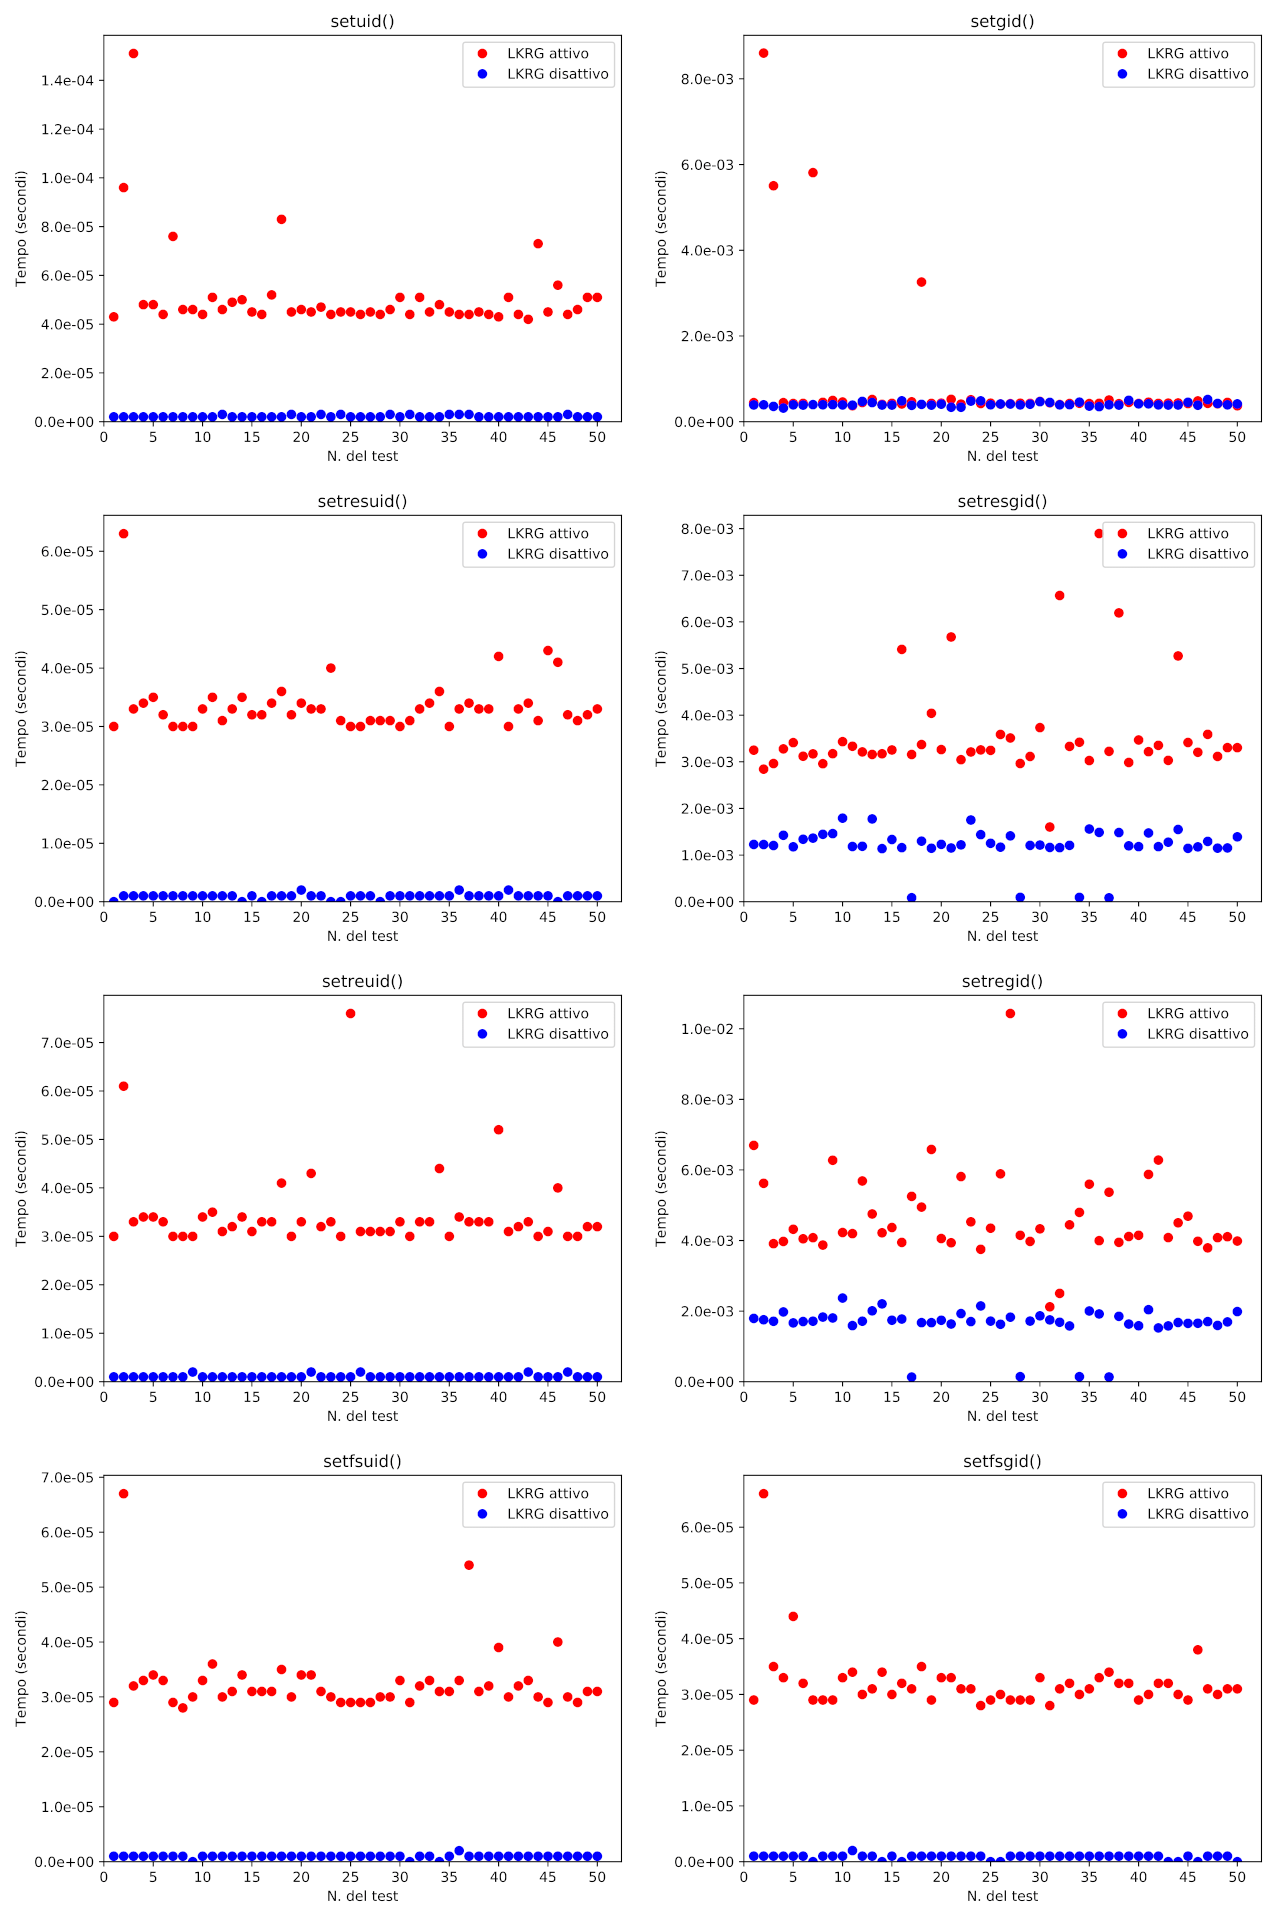
\includegraphics[scale=1.15]{Figures/Ubuntu/SingleSet}
\caption[Benchmark funzioni \emph{setX} con ncycle=1 (Ubuntu)]{Benchmark funzioni \emph{setX} con ncycle=1 (Ubuntu).}
\label{fig:setxUbuntuFig}
\end{figure}

Nella \autoref{fig:setxUbuntuFig} sono mostrati i risultati dei test delle funzionalità indicate con \emph{setX()} che alterano i parametri del processo, dove X è il parametro stesso (esempio: uid). Si noti come l'unica system call il cui tempo d'esecuzione non è rilevantemente influenzato dalla presenza di LKRG sia la \emph{setgid()}, i cui risultati mostrano come rimanga circa costante ad eccezione di qualche test.

Per tutte le altre funzioni, si osserva che la differenza del tempo d'esecuzione con il modulo caricato e modulo non caricato è elevata, passando da un'ordine di grandezza pari a $10^{-6} \approx 0$ nel grafico a $10^{-5}$ tranne nella \emph{setregid()} e \emph{setresgid()} in cui il tempo aumenta ma di fattore $\approx 2$. Tali tempi per il calcolatore sono pressappoco irrilevanti, nonostante graficamente possano avere un impatto diverso e si potrebbe pensare che sia totalmente sconsigliato l'utilizzo di LKRG. Di seguito è riportata la tabella in cui vengono indicate la media e la deviazione standard per ognuna delle system call nel grafico. 

\begin{table}[!htbp]
\centering
\begin{tabular}{|c|c|c|c|c|}
\hline
\textbf{SystemCall} & \bm{$\overline{x}$} \textbf{loaded} & \bm{$\overline{x}$} \textbf{unloaded} & \bm{$\sigma$} \textbf{loaded} & \bm{$\sigma$} \textbf{unloaded}\\
\hline
setuid() & 5.130e-05 & 2.200e-06 & 1.763e-05 & 4.000e-07 \\
\hline
setgid() & 8.679e-04 & 4.079e-04 & 1.549e-03 & 4.176e-05 \\
\hline
setresuid() & 3.366e-05 & 9.200e-07 & 5.152e-06 & 4.400e-07 \\
\hline
setresgid() & 3.577e-03 & 1.210e-03 & 1.052e-03 & 3.700e-04 \\
\hline
setreuid() & 3.458e-05 & 1.100e-06 & 8.183e-06 & 3.000e-07 \\
\hline
setregid() & 4.652e-03 & 1.646e-03 & 1.234e-03 & 4.758e-04 \\
\hline
setfsuid() & 3.270e-05 & 9.600e-07 & 6.306e-06 & 2.800e-07 \\
\hline
setfsgid() & 3.212e-05 & 8.400e-07 & 5.548e-06 & 4.176e-07 \\
\hline
\end{tabular}
\caption{Dati benchmark funzioni \emph{setX} con ncycle=1 (Ubuntu)}
\label{table:setxUbuntuData}
\end{table}

Si osservi l'enorme differenza che vi è non solo tra il tempo medio della singola chiamata, ma anche tra la deviazione standard, ovvero l'indice di dispersione statistico che indica quanto mediamente i dati si discostano dalla media stessa. La differenza tra la deviazione standard con LKRG caricato e non è sempre almeno di un ordine di grandezza, ad eccezione della prima funzione in cui è persino due ordini. L'incremento dei tempi d'esecuzione delle system call suggeriscono l'effettivo intervento del modulo, il quale compiendo i propri controlli d'integrità aggiunge sicuramente ulteriore tempo alla chiamata a funzione.

I grafici in \autoref{fig:othersUbuntuFig} e i dati nella \autoref{table:othersUbuntuData} riportano i risultati delle restanti system call testate nelle stesse medesime condizioni. Mentre i grafici delle funzionalità \emph{open()}, \emph{fork()} e \emph{delete\_module()} presentano una distribuzione dei dati simili a quelle analizzate in precedenza, quella della \emph{insert\_module()} è molto differente, in quanto i tempi variano ragionevolmente in entrambe le situazioni di testing. Mediamente il tempo d'esecuzione con LKRG è superiore, ma come si può notare talvolta può impiegare più tempo quando il modulo non è presente, in quanto incidono numerosi fattori nell'esecuzione di questa chiamata legati al caricamento dinamico di un modulo nel kernel; infatti è interessante osservare che la deviazione standard misurata è maggiore quando il modulo non è caricato. È dunque possibile, come nel nostro caso, che nonostante LKRG sia attivo il sistema impieghi meno tempo a caricare un modulo rispetto a quando non lo sia.

\begin{table}[!htbp]
\centering
\begin{tabular}{|c|c|c|c|c|}
\hline
\textbf{SystemCall} & \bm{$\overline{x}$} \textbf{loaded} & \bm{$\overline{x}$} \textbf{unloaded} & \bm{$\sigma$} \textbf{loaded} & \bm{$\sigma$} \textbf{unloaded}\\
\hline
open() & 3.398e-05 & 1.100e-06 & 5.006e-06 & 3.000e-07 \\
\hline
fork() & 3.518e-05 & 1.260e-06 & 4.117e-06 & 4.386e-07 \\
\hline
execve() & 7.740e-06 & 6.300e-06 & 2.234e-06 & 1.389e-06 \\
\hline
insert\_module() & 9.532e-02 & 6.940e-02 & 1.180e-02 & 1.587e-02 \\
\hline
delete\_module() & 3.226e-05 & 9.400e-07 & 4.837e-06 & 4.200e-07 \\
\hline
\end{tabular}
\caption{Dati benchmark restanti funzioni con ncycle=1 (Ubuntu)}
\label{table:othersUbuntuData}
\end{table}

\begin{figure}[!ht]
\centering
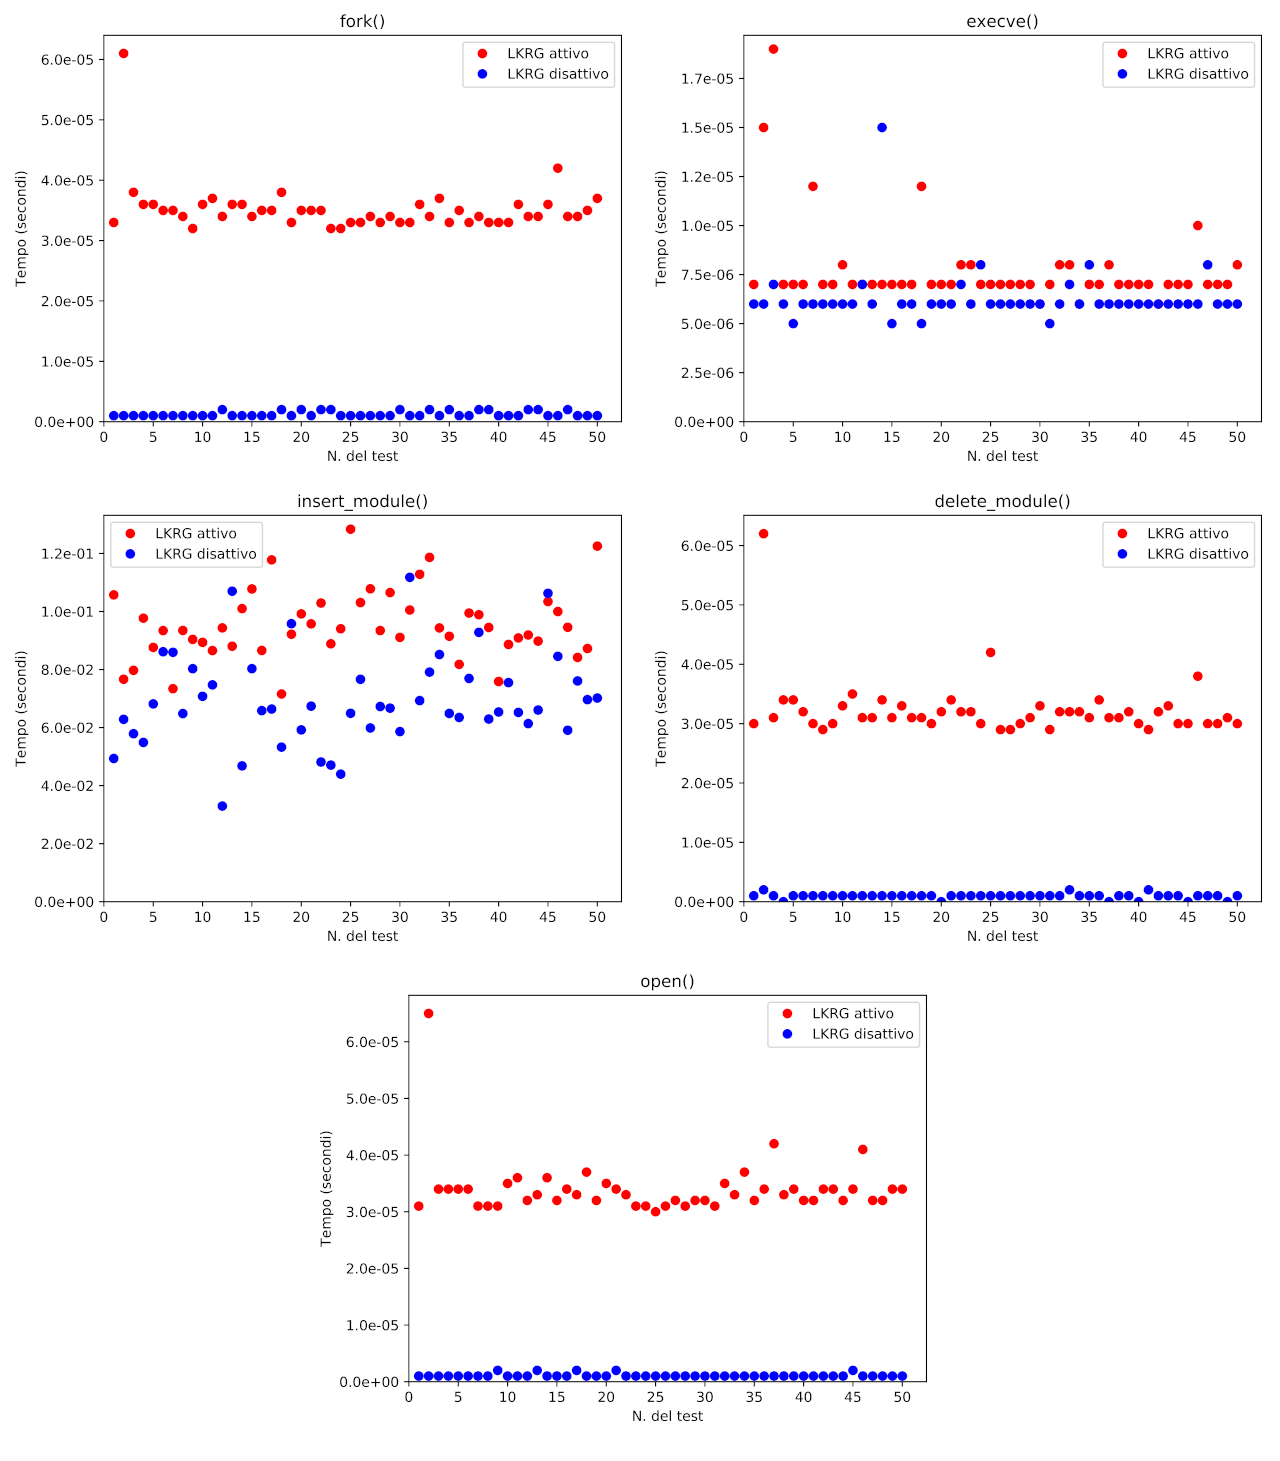
\includegraphics[scale=1.3]{Figures/Ubuntu/SingleOthers}
\caption[Benchmark restanti system call con ncycle=1 (Ubuntu)]{Benchmark restanti system call con ncycle=1 (Ubuntu).}
\label{fig:othersUbuntuFig}
\end{figure}

Anche la \emph{execve()} ha un range di valori differenti dalle altre system call, nonostante la distribuzione sia molto simile. Sicuramente LKRG aggiunge del tempo effettuando i suoi controlli, ma la parte più consistente di questa funzione è il reset di memoria del processo corrente, effettuando la sovrascrittura delle vecchie risorse con delle nuove dedicate al comando indicato come parametro. È dunque possibile, come nel nostro caso, che nonstante LKRG sia attivo il sistema impieghi meno tempo ad allocare le risorse al nuovo processo, per vari motivi di scheduling, disponibilità delle risorse o ottimizzazioni. Mediamente si può affermare che il tempo misurato con LKRG è superiore di circa il 22\% il tempo misurato senza.

In generale i dati nella \autoref{table:othersUbuntuData} sono consistenti con quelli nella \autoref{table:setxUbuntuData}: il tempo di certe funzionalità come la rimozione del modulo cambia di fattore $\approx 10$, mentre in altre la differenza è minore.
\\\par

Analizziamo ora come cambiano i tempi d'esecuzione lanciando singolarmente il programma SysBench con ncycle=1, 10, 100, 1000 e 10000 per capire perchè i risultati medi ottenuti possano essere così diversi rispetto a più esecuzioni con lo stesso parametro. Più semplicemente, la differenza tra le due esecuzioni si può riassumere nei seguenti comandi:

\begin{itemize}
\item \emph{sudo ./script.sh 10000 1 path/to/p\_lkrg.jo}, dove 10000 sono le volte che verrà richiamato il programma Sysbench e 1 corrisponde al parametro ncycle;
\item \emph{sudo ./sysbench 10000 filename}.
\end{itemize} 

Senza consultare alcun risultato, possiamo aspettarci di ottenere due output differenti, influenzati dalle ottimizzazioni del processore. L'obiettivo dunque è verificare che il valore della singola system call misurato richiamandola 10000 volte all'interno dello stesso programma sia effettivamente inferiore della media dei valori ottenuti mediante 10000 esecuzioni in cui viene eseguita una volta sola.

\begin{figure}[!ht]
\centering
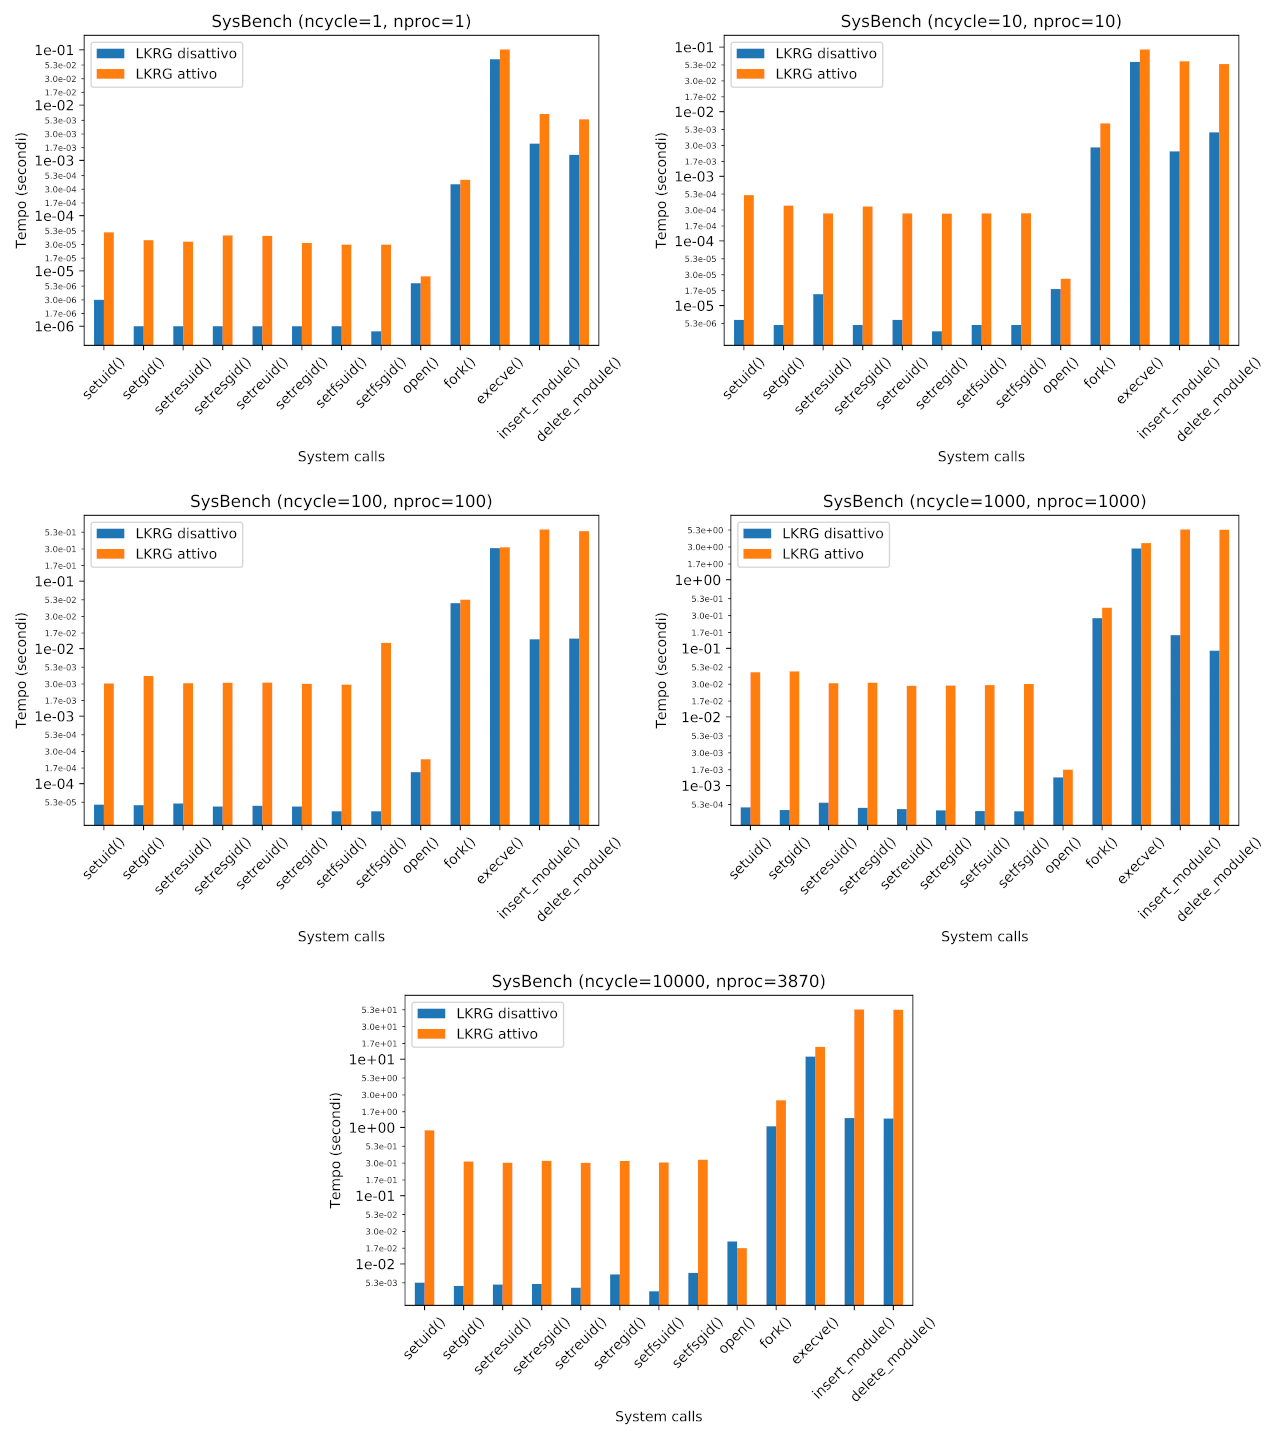
\includegraphics[scale=1.4]{Figures/Ubuntu/Total}
\caption[Benchmark tempo totale (Ubuntu)]{Benchmark tempo totale (Ubuntu).}
\label{fig:totUbuntuFig}
\end{figure}

Iniziamo commentando la \autoref{fig:totUbuntuFig}, raffigurante il tempo totale d'esecuzione delle system call nelle 5 esecuzioni con ncycle differente. Per l'asse delle ordinate (y) si è utilizzato una scala logaritmica, al fine di riuscire ad inserire tutti i dati nello stesso grafico, sebbene siano molto discostanti tra loro.

Si può osservare il tempo aggiunto dalla presenza di LKRG semplicemente sottraendo alle barre arancioni le corrispettive blu. In quasi tutte le funzioni ad eccezione della \emph{fork()}, \emph{execve()} e \emph{open()} l'overhead aggiunto dal modulo è significativo ed aumenta sempre di più al variare del numero di chiamate. È da premettere che tali test sono specifici per questa analisi, al fine di comprendere il lavoro del modulo LKRG, ma in una situazione reale è altamente improbabile trovare un programma che effettui così tante volte consecutive la medesima chiamata.

L'unica che potrebbe raffigurare uno scenario reale è la \emph{open()}, in quanto moltissimi programmi lavorano con più file, aprendoli e chiudendoli diverse volte, ma i grafici e le tabelle presenti in questa trattazione suggeriscono che tale system call sia leggermente influenzata da LKRG a differenza di molte altre, tra cui la \emph{insert\_module()}. Infatti quest'ultima funzione e la sua opposta \emph{delete\_module()} risentono dei controlli d'integrità, aumentando il loro tempo d'esecuzione di circa mezzo ordine di grandezza; se nei primi grafici i loro tempi con LKRG attivo sono inferiori a quelli della \emph{execve()}, negli ultimi in cui ncycle è molto più grande superano qualsiasi tempo d'esecuzione delle altre system call, in quanto si somma ncycle-volte l'overhead aggiunto dal modulo, il quale risulta essere massimo per queste due funzioni. Infine, un'altra differenza facile da notare sono i tempi delle funzioni \emph{setX}; nonostante essi siano molto più piccoli delle altre funzionalità, si può affermare che in percentuale sono quelle maggiormente influenzate, in quanto il rapporto tra i tempi è pari a $1.5x10^{1}$ per la \emph{setuid()} e persino maggiore per le altre.

\begin{table}[!htbp]
\centering
\begin{tabular}{|c|c|c|c|c|}
\hline
\textbf{SystemCall} & \bm{$\overline{x}$} \textbf{loaded} & \bm{$\overline{x}$} \textbf{unloaded} & \bm{$\sigma$} \textbf{loaded} & \bm{$\sigma$} \textbf{unloaded}\\
\hline
setuid() & 5.349e-05 & 1.021e-06 & 2.007e-05 & 9.903e-07 \\
\hline
setgid() & 3.772e-05 & 5.793e-07 & 4.858e-06 & 2.112e-07 \\
\hline
setresuid() & 3.059e-05 & 8.148e-07 & 2.326e-06 & 3.895e-07 \\
\hline
setresgid() & 3.467e-05 & 5.885e-07 & 4.780e-06 & 2.065e-07 \\
\hline
setreuid() & 3.197e-05 & 5.945e-07 & 5.749e-06 & 2.102e-07 \\
\hline
setregid() & 2.994e-05 & 6.001e-07 & 2.144e-06 & 2.269e-07 \\
\hline
setfsuid() & 2.919e-05 & 5.426e-07 & 1.369e-06 & 2.319e-07 \\
\hline
setfsgid() & 4.847e-05 & 5.724e-07 & 3.667e-05 & 1.707e-07 \\
\hline
open() & 3.263e-06 & 2.547e-06 & 2.394e-06 & 1.749e-06 \\
\hline
fork() & 5.349e-04 & 3.333e-04 & 1.067e-04 & 7.851e-05 \\
\hline
execve() & 2.428e-02 & 1.645e-02 & 3.877e-02 & 2.558e-02 \\
\hline
insert\_module() & 5.907e-03 & 5.380e-04 & 5.558e-04 & 7.400e-04 \\
\hline
delete\_module() & 5.430e-03 & 4.213e-04 & 8.738e-05 & 4.404e-04 \\
\hline
\end{tabular}
\caption{Dati benchmark con ncycle=1, 10, 100, 1000, 10000 (Ubuntu)}
\label{table:totUbuntuData}
\end{table}

Confrontando i dati della \autoref{table:totUbuntuData} con quelli delle tabelle ottenute precedentemente (\autoref{table:othersUbuntuData} e \autoref{table:setxUbuntuData}) si osserva l'enorme differenza del tempo medio d'esecuzione (\bm{$\overline{x}}$) delle funzioni in entrambi i casi, potendo pensare che vi sia un errore nella misurazione. In realtà la differenza è dovuta all'insieme delle ottimizzazioni apportate dal processore e dalla memoria cache non trattate in questo elaborato. Una buona idea per uno possibile sviluppo è quella di estendere la trattazione analizzando il comportamento del modulo in processori differenti, capendo le modifiche apportate da ognuno analizzando ogni singolo step d'esecuzione del programma. Non essendo il processore e il compilatore argomenti di tesi, mi limito a mostrare qualche grafico interessante per capire come il tempo medio della singola system call cambi a seconda del numero di volte che viene invocata all'interno del medesimo programma.

\begin{figure}[!htbp]
\centering
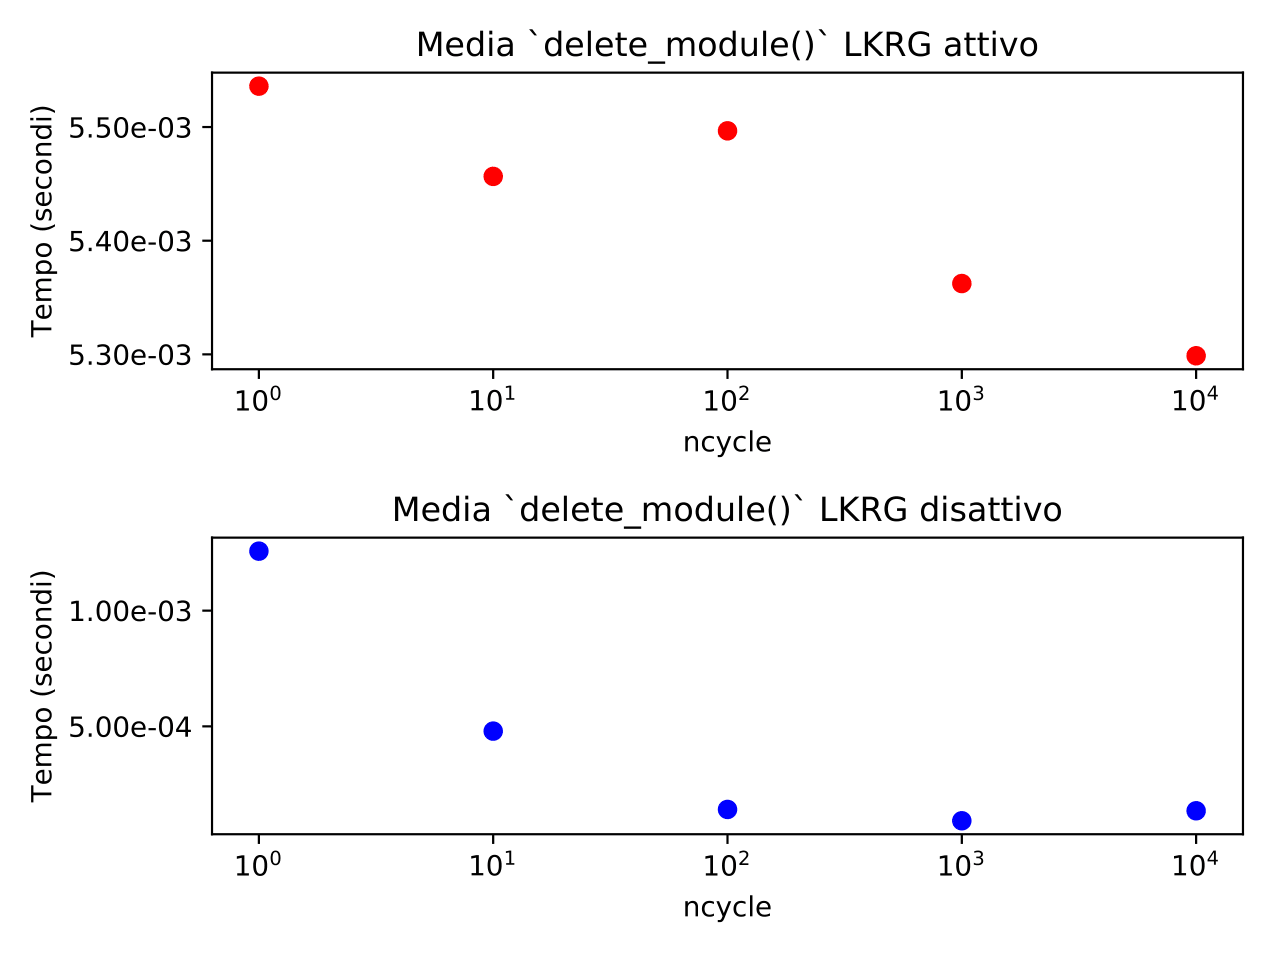
\includegraphics[scale=0.18]{Figures/Ubuntu/Mean1}
\caption[Media singole system call nei 5 benchmark parte 1 (Ubuntu)]{Media singole system call nei 5 benchmark parte 1 (Ubuntu).}
\label{fig:mean1UbuntuFig}
\end{figure}

\begin{figure}[!htbp]
\centering
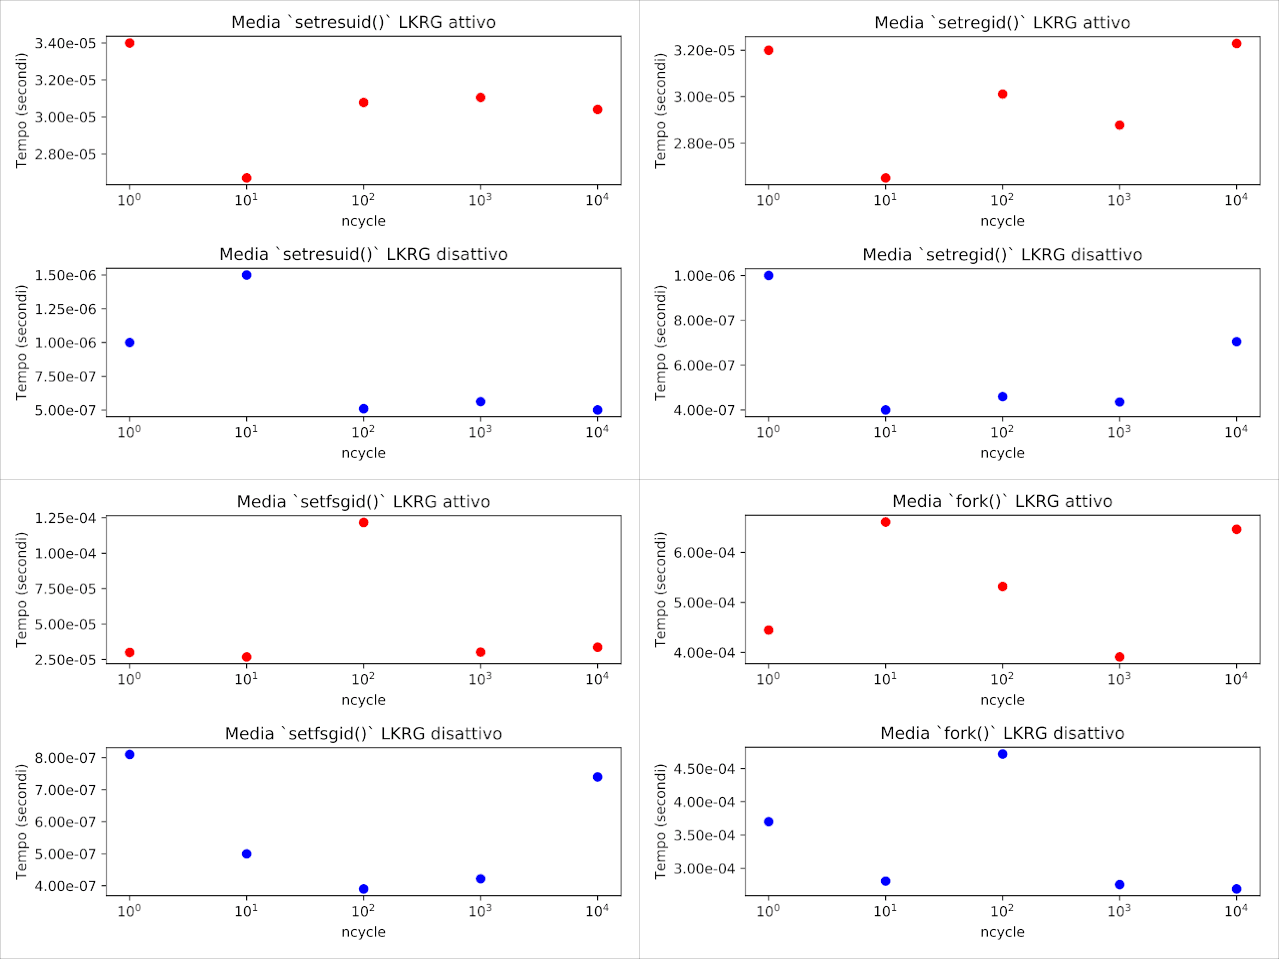
\includegraphics[scale=1.3]{Figures/Ubuntu/Mean2}
\caption[Media singole system call nei 5 benchmark parte 2 (Ubuntu)]{Media singole system call nei 5 benchmark parte 2 (Ubuntu).}
\label{fig:mean2UbuntuFig}
\end{figure}

\begin{figure}[!htbp]
\centering
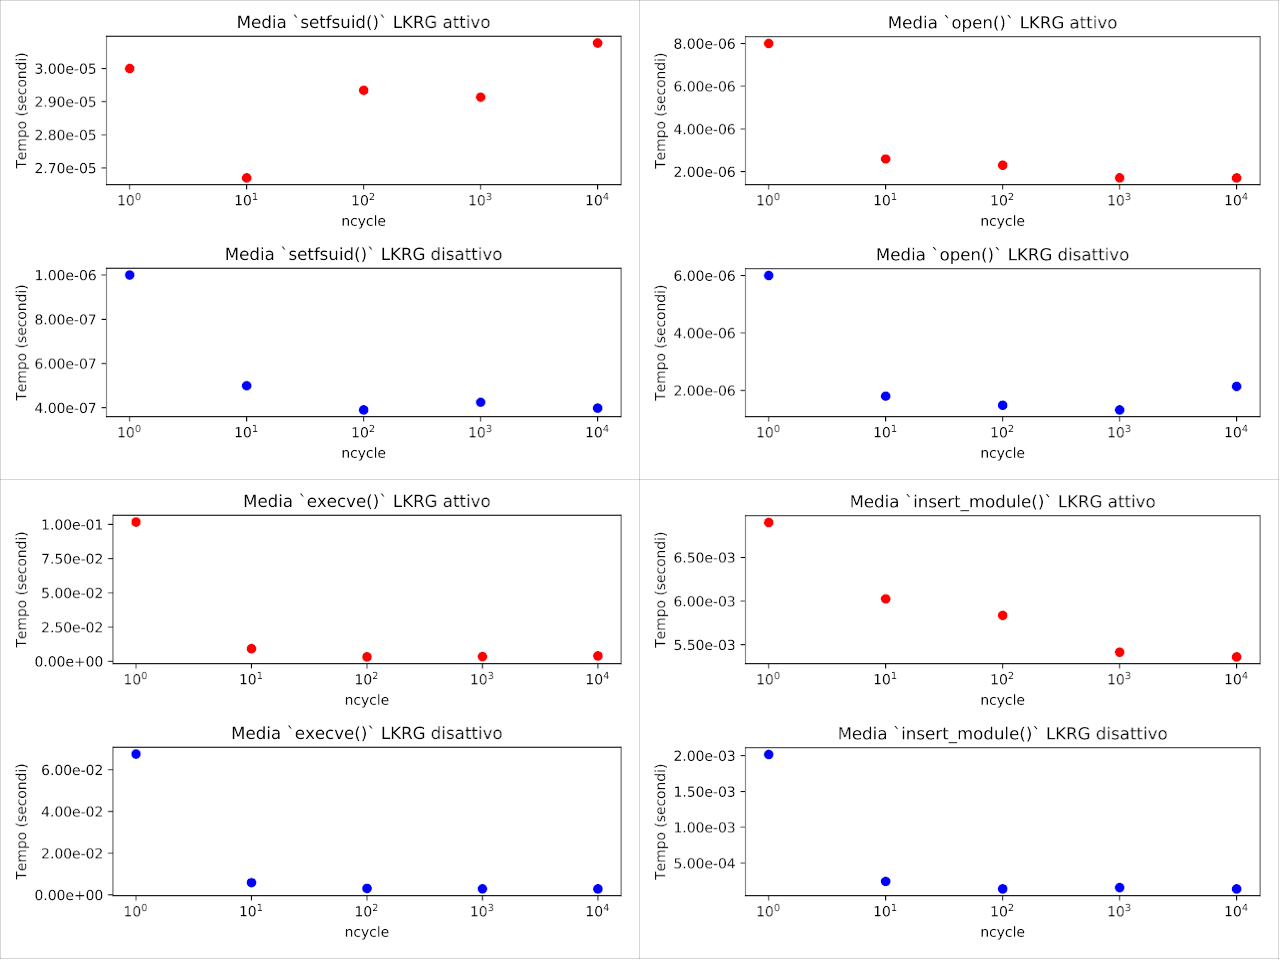
\includegraphics[scale=1.3]{Figures/Ubuntu/Mean3}
\caption[Media singole system call nei 5 benchmark parte 3 (Ubuntu)]{Media singole system call nei 5 benchmark parte 3 (Ubuntu).}
\label{fig:mean3UbuntuFig}
\end{figure}

\begin{figure}[!htbp]
\centering
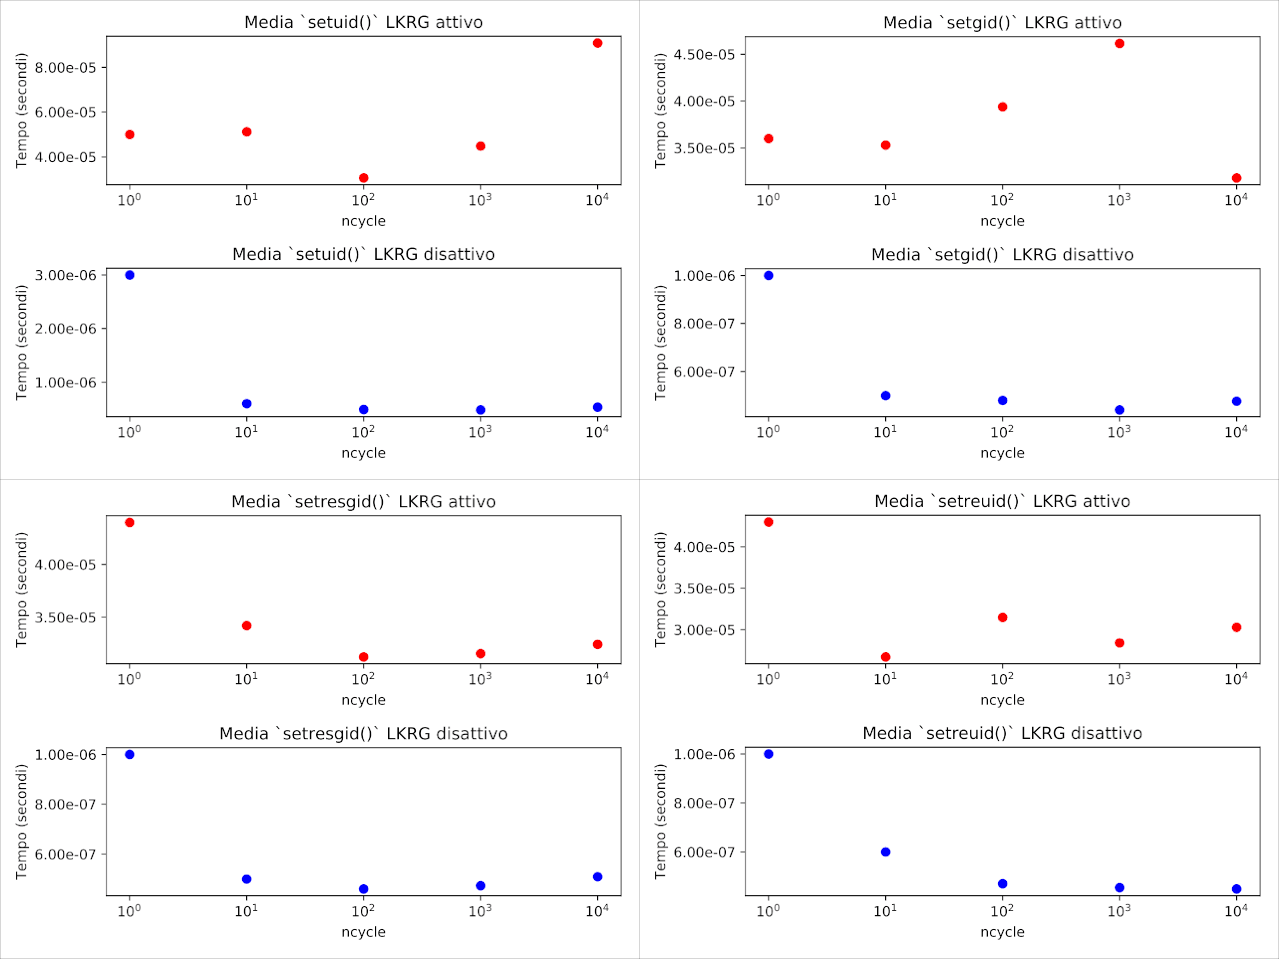
\includegraphics[scale=1.3]{Figures/Ubuntu/Mean4}
\caption[Media singole system call nei 5 benchmark parte 4 (Ubuntu)]{Media singole system call nei 5 benchmark parte 4 (Ubuntu).}
\label{fig:mean4UbuntuFig}
\end{figure}

Ad eccezione dei grafici in \autoref{fig:mean4UbuntuFig} che presentano valori oscillanti, nei restanti è chiaro l'intervento di un ottimizzatore, grazie al quale in base a quante chiamate vengono effettuate il tempo d'esecuzione medio della singola system call diminuisce in maniera esponenziale. Come scala per l'asse delle x è stata utilizzata una scala logaritmica per rappresentare il numero tutti i valori assunti da ncycle.

%----------------------------------------------------------------------------------------
%	DEBIAN TESTS
%----------------------------------------------------------------------------------------
\section{Test in Debian}

In questa sezione sono presentati i risultati della valutazione della seconda distribuzione presa in analisi: Debian. I test in questo ambiente, nonostante presentino varie similitudini con i risultati ottenuti in Ubuntu, suggeriscono un'ottima risposta del sistema al caricamento di LKRG.

Per seguire la stessa logica di presentazione della sezione precedente, iniziamo commentando i risultati ottenuti in seguito a 50 esecuzioni di SysBench con parametro ncycle=1 presentati nei seguenti grafici.

\begin{figure}[!ht]
\centering
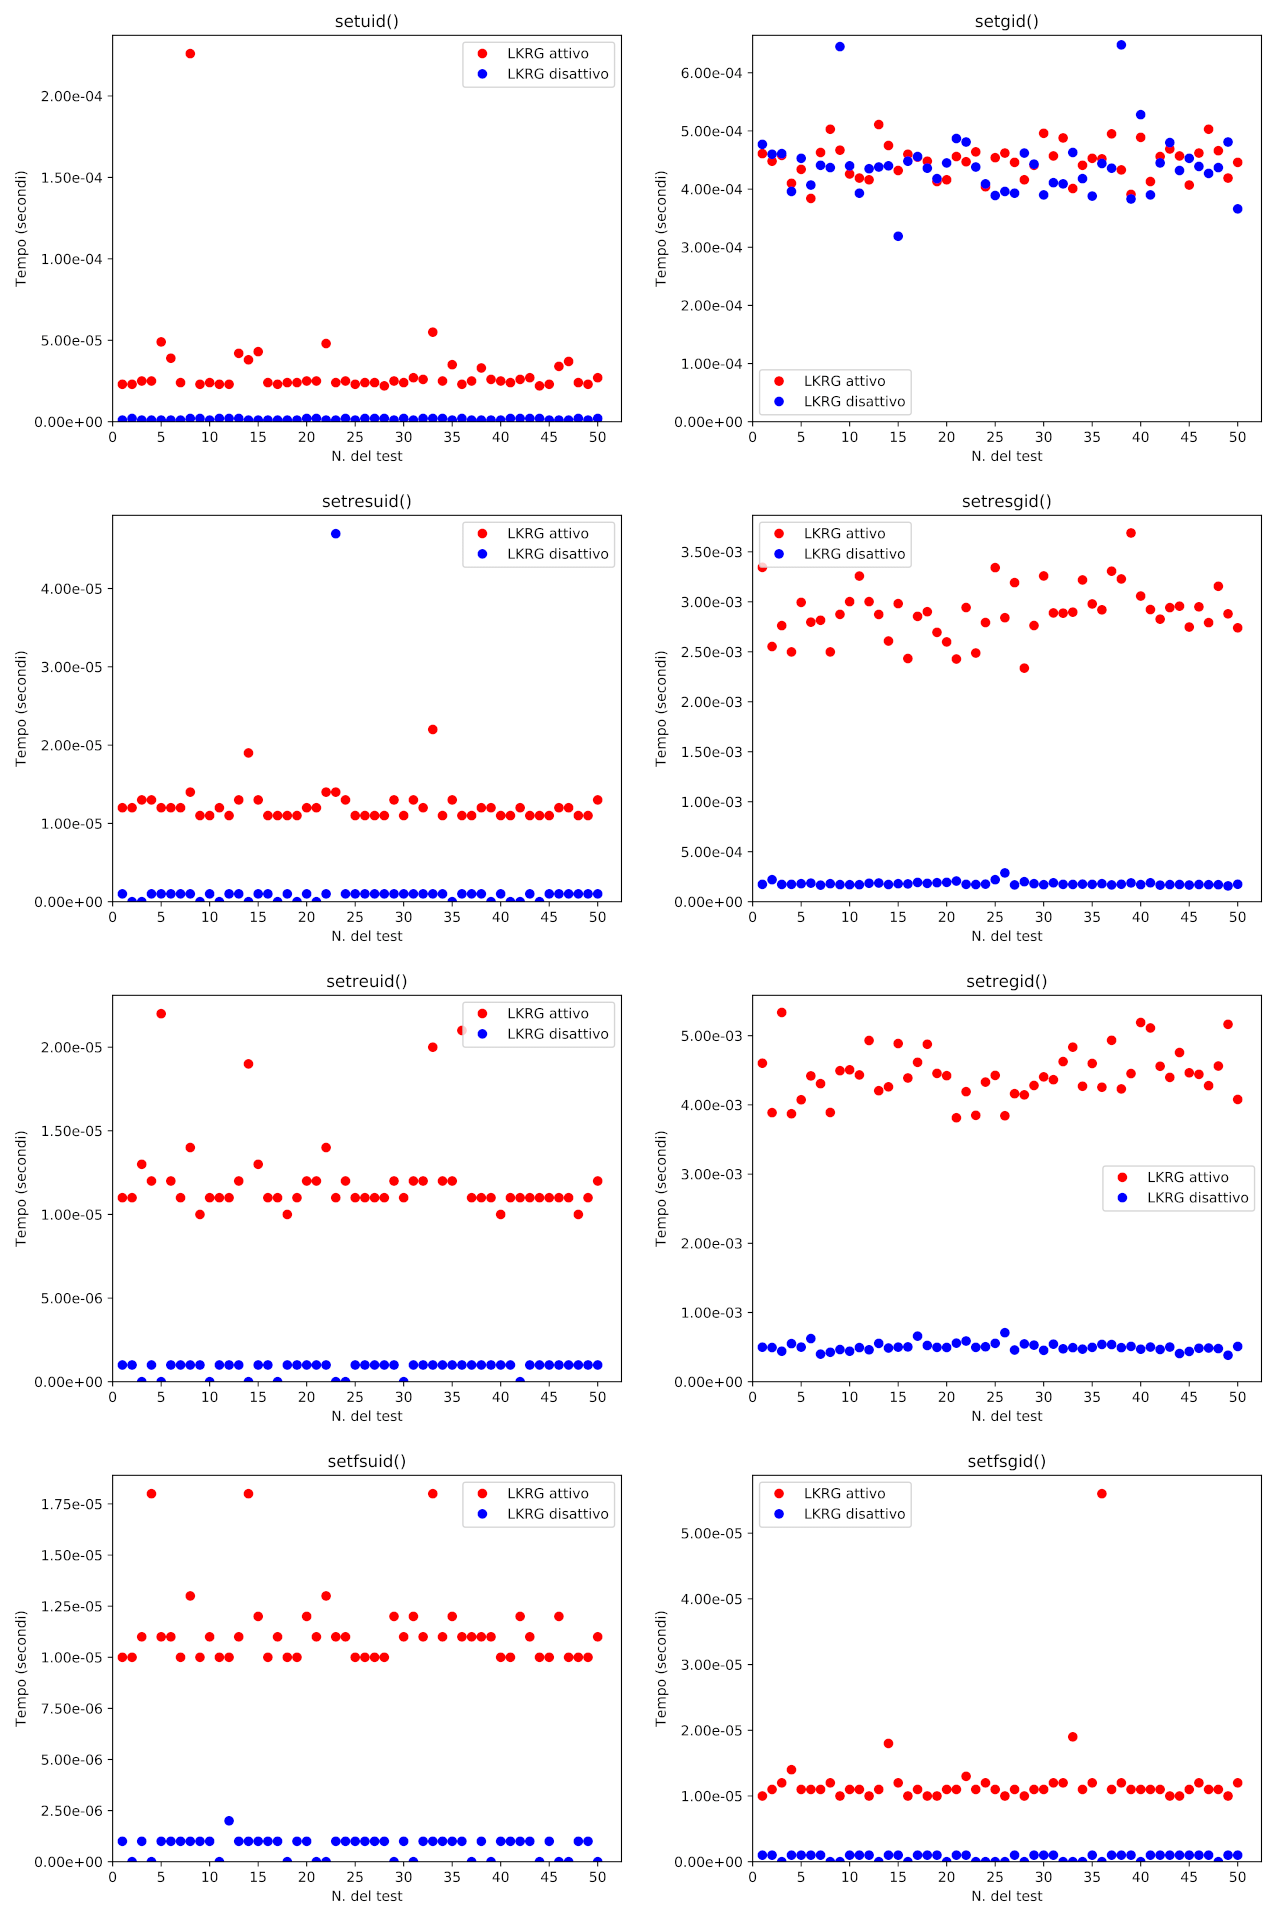
\includegraphics[scale=1.3]{Figures/Debian/SingleSet}
\caption[Benchmark funzioni \emph{setX} con ncycle=1 (Debian)]{Benchmark funzioni \emph{setX} con ncycle=1 (Debian).}
\label{fig:setxDebianFig}
\end{figure}

Come si può osservare in \autoref{fig:setxDebianFig} è chiara la differenza tra i tempi d'esecuzione delle varie system e l'overhead aggiunto da LKRG. Nonostante la dispersione dei grafici sia simile a quelli presentati per Ubuntu, cambia il range dei tempi d'esecuzione: ad esempio per la \emph{setresgid()} osserviamo che i tempi misurati senza il modulo attivo sono di due ordini di grandezza più piccoli rispetto a quelli con LKRG presente, mentre in Ubuntu la differenza è minima, cambia solamente un fattore di proporzionalità pari a 3.
La system call che risulta essere meno influenzata anche in ambiente Debian risulta essere la \emph{setgid()}, i cui valori oscillano in un intorno di $1x10^{-4}$ che rispetto ai tempi misurati è relativamente piccolo. Esclusa questa system call e la \emph{setresuid()}, i cui test rivelano qualche rallentamento nell'esecuzione della funzione anche senza LKRG, nei grafici di tutte le altre funzionalità si osserva che mentre in presenza del modulo i tempi campionati sono molto più variabili e dispersi, in sua assenza i valori risultano essere più omogenei ed allineati, sebbene vi sia qualche differenza ma in grandezza minore.

\begin{table}[!htbp]
\centering
\begin{tabular}{|c|c|c|c|c|}
\hline
\textbf{SystemCall} & \bm{$\overline{x}$} \textbf{loaded} & \bm{$\overline{x}$} \textbf{unloaded} & \bm{$\sigma$} \textbf{loaded} & \bm{$\sigma$} \textbf{unloaded}\\
\hline
setuid() & 3.202e-05 & 1.460e-06 & 2.877e-05 & 4.984e-07 \\
\hline
setgid() & 4.477e-04 & 4.402e-04 & 2.982e-05 & 5.500e-05 \\
\hline
setresuid() & 1.220e-05 & 1.660e-06 & 1.949e-06 & 6.492e-06 \\
\hline
setresgid() & 2.894e-03 & 1.812e-04 & 2.685e-04 & 1.971e-05 \\
\hline
setreuid() & 1.212e-05 & 8.200e-07 & 2.628e-06 & 3.842e-07 \\
\hline
setregid() & 4.438e-03 & 5.018e-04 & 3.587e-04 & 5.863e-05 \\
\hline
setfsuid() & 1.124e-05 & 7.400e-07 & 1.893e-06 & 4.821e-07 \\
\hline
setfsgid() & 1.228e-05 & 6.600e-07 & 6.465e-06 & 4.737e-07 \\
\hline
\end{tabular}
\caption{Dati benchmark funzioni \emph{setX} con ncycle=1 (Debian)}
\label{table:setxDebianData}
\end{table}

Dalla \autoref{table:setxDebianData} si evince quanto appena commentato: concentrandosi sulla deviazione standard in entrambe le situazioni, confermiamo appunto che i valori sono più concentrati ed omogenei quando LKRG non è presente nel sistema, mentre una volta caricato i tempi misurati variano in maniera più evidente. Si può affermare dunque che i controlli d'integrità, sebbene non comportino un aumento eccessivo della chiamata, influenzino in maniera variabile l'esecuzione. Per fare un esempio si considerino i dati relativi alla \emph{setuid()}: una deviazione standard di $2.877x10^{-5}$ con LKRG presente è accettabile rispetto alla media $3.202x10^{-5}$ delle chiamate, ma se la si confronta con i valori misurati in assenza del modulo risulta essere non trascurabile, in quanto la deviazione è dell'ordine del $10^{-7}$. È necessario prima di giungere a conclusioni considerare questi fattori e queste differenze negli ordini di grandezza dei dati, in modo da comprendere e confrontare con coerenza la variazione dei tempi d'esecuzione delle funzioni.
\\\par

\begin{figure}[!ht]
\centering
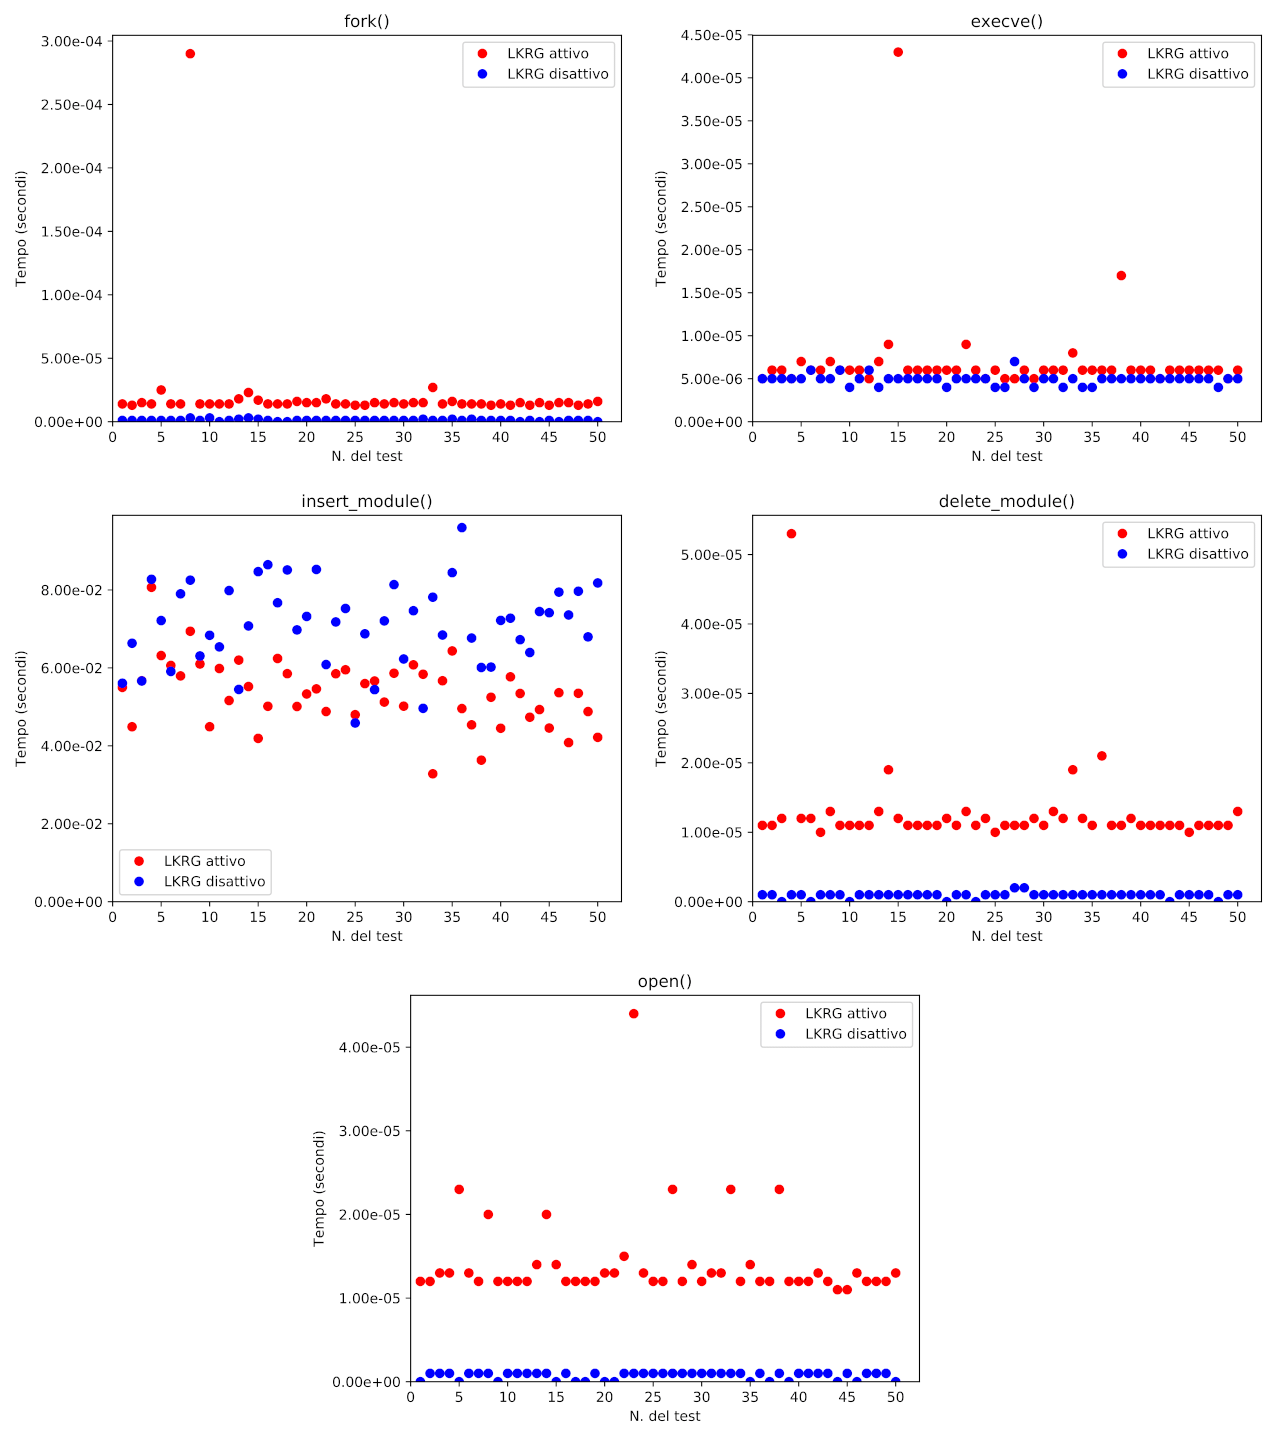
\includegraphics[scale=1.4]{Figures/Debian/SingleOthers}
\caption[Benchmark restanti funzioni con ncycle=1 (Debian)]{Benchmark restanti funzioni con ncycle=1 (Debian).}
\label{fig:othersDebianFig}
\end{figure}

Sorprendentemente, il grafico della \emph{execve()} in \autoref{fig:othersDebianFig} rivela che il tempo d'esecuzione è minore quando misurato con il modulo presente, mentre risulta essere leggermente maggiore nel caso opposto, inducendo a concludere che tale system call non sia influenzata da LKRG. La scala dei valori in tale grafico risulta essere meno estesa, suggerendo dunque più omogeneità nei dati rispetto agli altri dove si può osservare che in ogni test delle funzionalità vi è sempre qualche valore che si discosta maggiormente dalla media. Ad esempio si consideri la \emph{fork()}: una misurazione è risultata essere di un'ordine di grandezza e mezzo più grande rispetto a tutte le altre, probabilmente dovuto a qualche ritardo nell'allocazione di risorse per il processo figlio da parte del programma e non a causa di LKRG. Ancora una volta si assiste ad un aumento di due ordini di grandezza del tempo d'esecuzione della \emph{open()} che, come in Ubuntu, varia da $7.200e^{-07}$ in assenza del modulo a $1.424e^{-05}$ una volta caricato.

\begin{table}[!htbp]
\centering
\begin{tabular}{|c|c|c|c|c|}
\hline
\textbf{SystemCall} & \bm{$\overline{x}$} \textbf{loaded} & \bm{$\overline{x}$} \textbf{unloaded} & \bm{$\sigma$} \textbf{loaded} & \bm{$\sigma$} \textbf{unloaded}\\
\hline
open() & 1.424e-05 & 7.200e-07 & 5.335e-06 & 4.490e-07 \\
\hline
fork() & 2.058e-05 & 1.080e-06 & 3.859e-05 & 6.882e-07 \\
\hline
execve() & 7.000e-06 & 4.900e-06 & 5.430e-06 & 5.745e-07 \\
\hline
insert\_module() & 5.349e-02 & 7.114e-02 & 8.344e-03 & 1.041e-02 \\
\hline
delete\_module() & 1.270e-05 & 9.000e-07 & 6.133e-06 & 4.123e-07 \\
\hline
\end{tabular}
\caption{Dati benchmark restanti funzioni con ncycle=1 (Debian)}
\label{table:othersDebianData}
\end{table}

\clearpage

Nella tabella \autoref{table:othersDebianData} si osservi come le system call \emph{open()} e \emph{delete\_module()} siano quelle più influenzate dal modulo, in quanto i valori medi si innalzano di fattore 1000, passando da tempi come $7.200e^{-07}$ e $9.000e-07$ a $1.424e-05$ e $1.270e-05$. Coerentemente con quanto detto in prececenza, non solo la media della singola chiamata alla funzione \emph{execve()} risulta essere leggermente maggiore in assenza del modulo, ma anche la deviazione standard (10 volte minore).
\\\par

\begin{figure}[!ht]
\centering
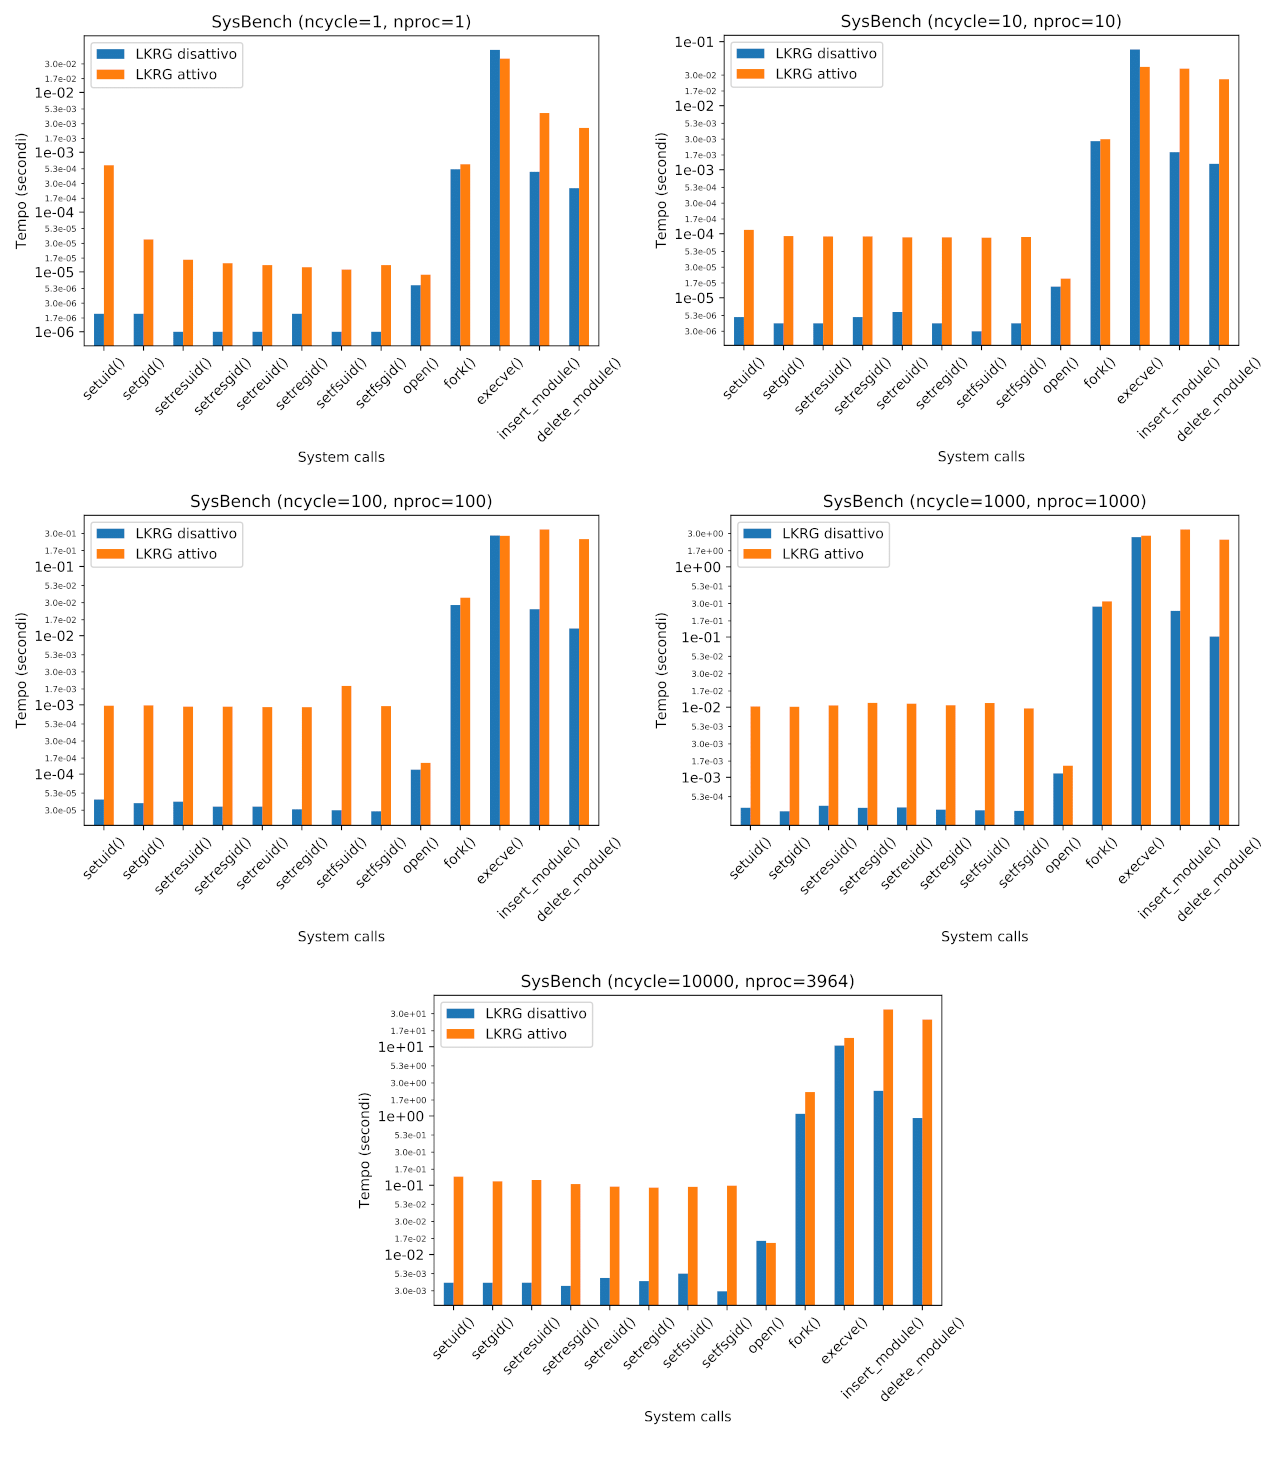
\includegraphics[scale=1.4]{Figures/Debian/Total}
\caption[Benchmark tempo totale (Debian)]{Benchmark tempo totale (Debian).}
\label{fig:totDebianFig}
\end{figure}

Procediamo ora con la medesima analisi effettuata in Ubuntu, ovvero il tempo d'esecuzione della singola system call nel caso venisse richiamata più volte all'interno del programma. Il test è stato effettuato ugualmente, con ncycle che assume i valori 1, 10, 100, 1000 e 10000 ed il sistema che si trova nello stesso stato in cui era la macchina Ubuntu. L'obiettivo è sempre quello di osservare il tempo medio d'esecuzione della singola system call per dedurre se anche in questo sistema vengono apportate ottimizzazioni.

In \autoref{fig:totDebianFig} si osserva il tempo totale d'esecuzione delle system call nei 5 scenari con ncycle differente. Iniziando a valutare il test con ncycle=1 che rappresenta inoltre i test discussi fino ad ora, si nota come LKRG influenzi maggiormente le funzioni \emph{setX()} e quelle inerenti alle operazioni con i moduli, le quali variano maggiormente rispetto alla \emph{open()}, \emph{fork() e la \emph{execve()}}. Quest'ultima soprattutto presenta tempi d'esecuzione maggiori in assenza del modulo nei test in cui viene richiamata un numero relativamente piccolo di volte, mentre più cresce ncycle più i due tempi tendono a differire per veramente poche unità sembrando quasi pareggianti. Vi è una lieve differenza anche nelle altre due funzionalità, le quali però mantengono il rapporto $\frac{Tattivo}{Tdisattivo}$ quasi costante. Sicuramente l'utente lanciando il programma è in grado di percepire la differenza d'esecuzione della \emph{insert\_module()} e \emph{delete\_module()}, in quanto in ordini di grandezza sono quelle con la differenza più alta (persino 30 volte più alta nei test con ncycle=10000), ma quelle che in percentuale al loro tempo d'esecuzione in assenza del modulo hanno subito maggiori rallentamenti sono le \emph{setX()} come già commentato.

\begin{table}[!htbp]
\centering
\begin{tabular}{|c|c|c|c|c|}
\hline
\textbf{SystemCall} & \bm{$\overline{x}$} \textbf{loaded} & \bm{$\overline{x}$} \textbf{unloaded} & \bm{$\sigma$} \textbf{loaded} & \bm{$\sigma$} \textbf{unloaded}\\
\hline
setuid() & 1.304e-04 & 7.380e-07 & 2.383e-04 & 6.326e-07 \\
\hline
setgid() & 1.512e-05 & 7.000e-07 & 9.966e-06 & 6.505e-07 \\
\hline
setresuid() & 1.142e-05 & 5.171e-07 & 2.494e-06 & 2.415e-07 \\
\hline
setresgid() & 1.089e-05 & 5.119e-07 & 1.766e-06 & 2.507e-07 \\
\hline
setreuid() & 1.038e-05 & 5.544e-07 & 1.544e-06 & 2.403e-07 \\
\hline
setregid() & 9.999e-06 & 6.941e-07 & 1.179e-06 & 6.540e-07 \\
\hline
setfsuid() & 1.188e-05 & 4.941e-07 & 3.586e-06 & 2.671e-07 \\
\hline
setfsgid() & 1.020e-05 & 4.634e-07 & 1.438e-06 & 2.712e-07 \\
\hline
open() & 3.077e-06 & 2.274e-06 & 2.969e-06 & 1.871e-06 \\
\hline
fork() & 4.332e-04 & 3.241e-04 & 1.349e-04 & 9.801e-05 \\
\hline
execve() & 9.963e-03 & 1.340e-02 & 1.345e-02 & 1.906e-02 \\
\hline
insert\_module() & 3.727e-03 & 2.734e-04 & 4.233e-04 & 1.006e-04 \\
\hline
delete\_module() & 2.510e-03 & 1.394e-04 & 5.203e-05 & 5.722e-05 \\
\hline
\end{tabular}
\caption{Dati benchmark con ncycle=1, 10, 100, 1000, 10000 (Debian)}
\label{table:totDebianData}
\end{table}

Tralasciando la precisione dei valori, l'analisi da effettuare è la medesima di quella inerente al sistema Ubuntu, ovvero da questa tabella si osservano valori che porterebbero a pensare ad un errore di misurazione. In realtà, osservando i grafici sottostanti si osserva come il tempo d'esecuzione medio delle singole system call diminuisca all'aumentare del numero di volte che vengono testate.

\clearpage

\begin{figure}[!htbp]
\centering
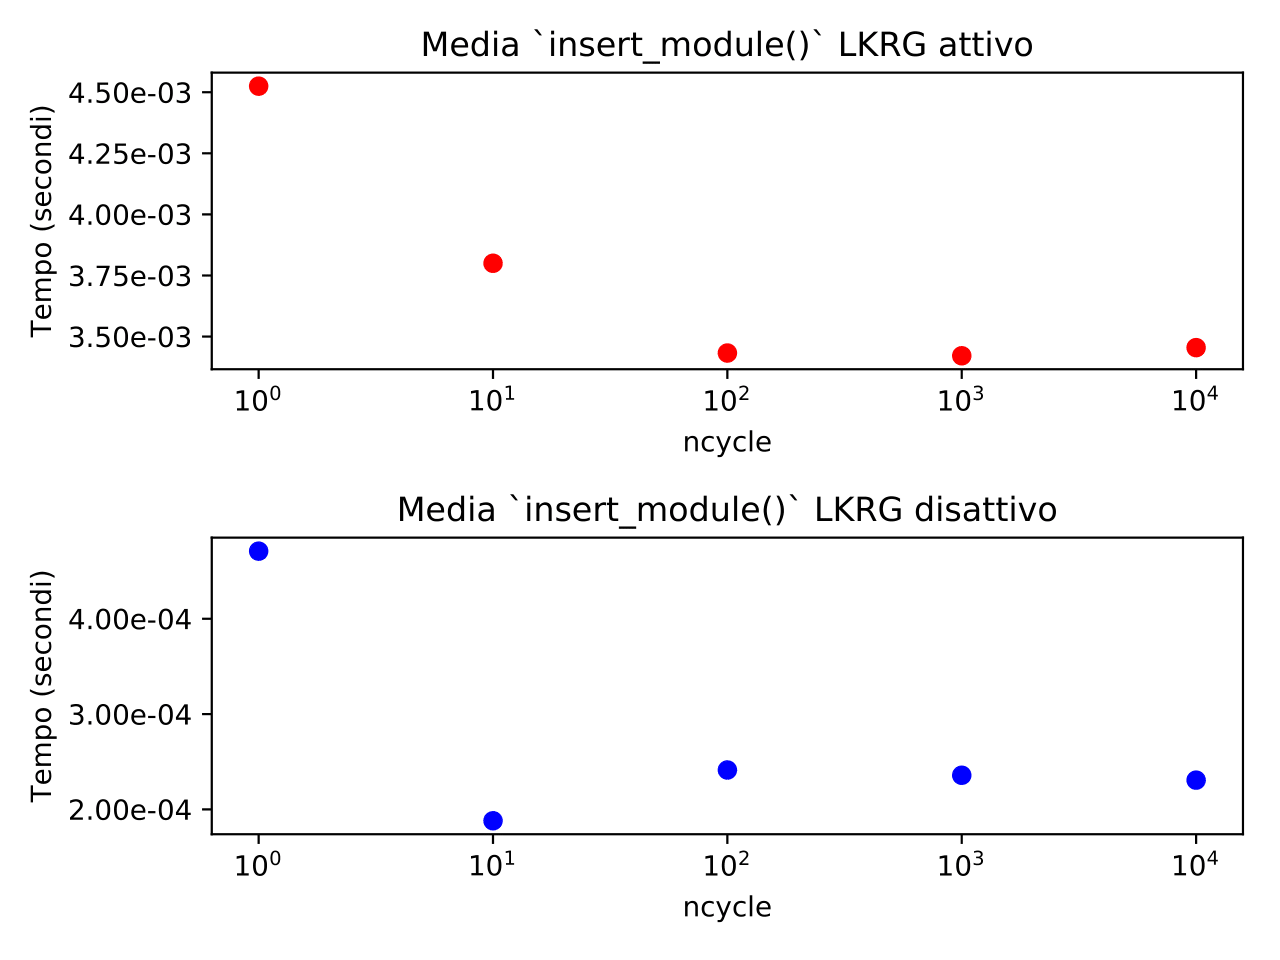
\includegraphics[scale=0.22]{Figures/Debian/Mean1}
\caption[Media singole system call nei 5 benchmark parte 1 (Debian)]{Media singole system call nei 5 benchmark parte 1 (Debian).}
\label{fig:mean1DebianFig}
\end{figure}

\begin{figure}[!htbp]
\centering
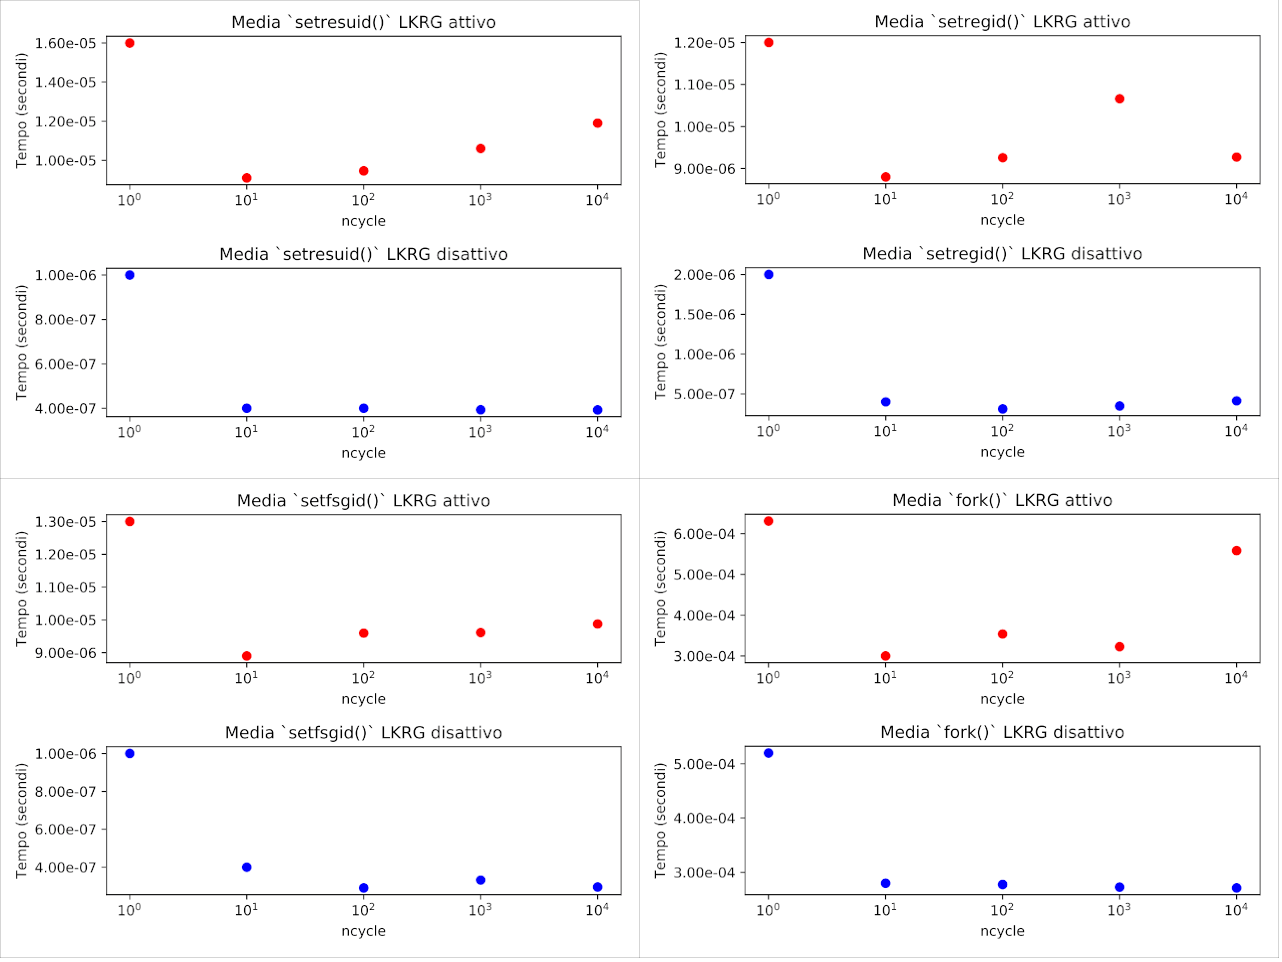
\includegraphics[scale=1.4]{Figures/Debian/Mean2}
\caption[Media singole system call nei 5 benchmark parte 2 (Debian)]{Media singole system call nei 5 benchmark parte 2 (Debian).}
\label{fig:mean2DebianFig}
\end{figure}

\clearpage

\begin{figure}[!htbp]
\centering
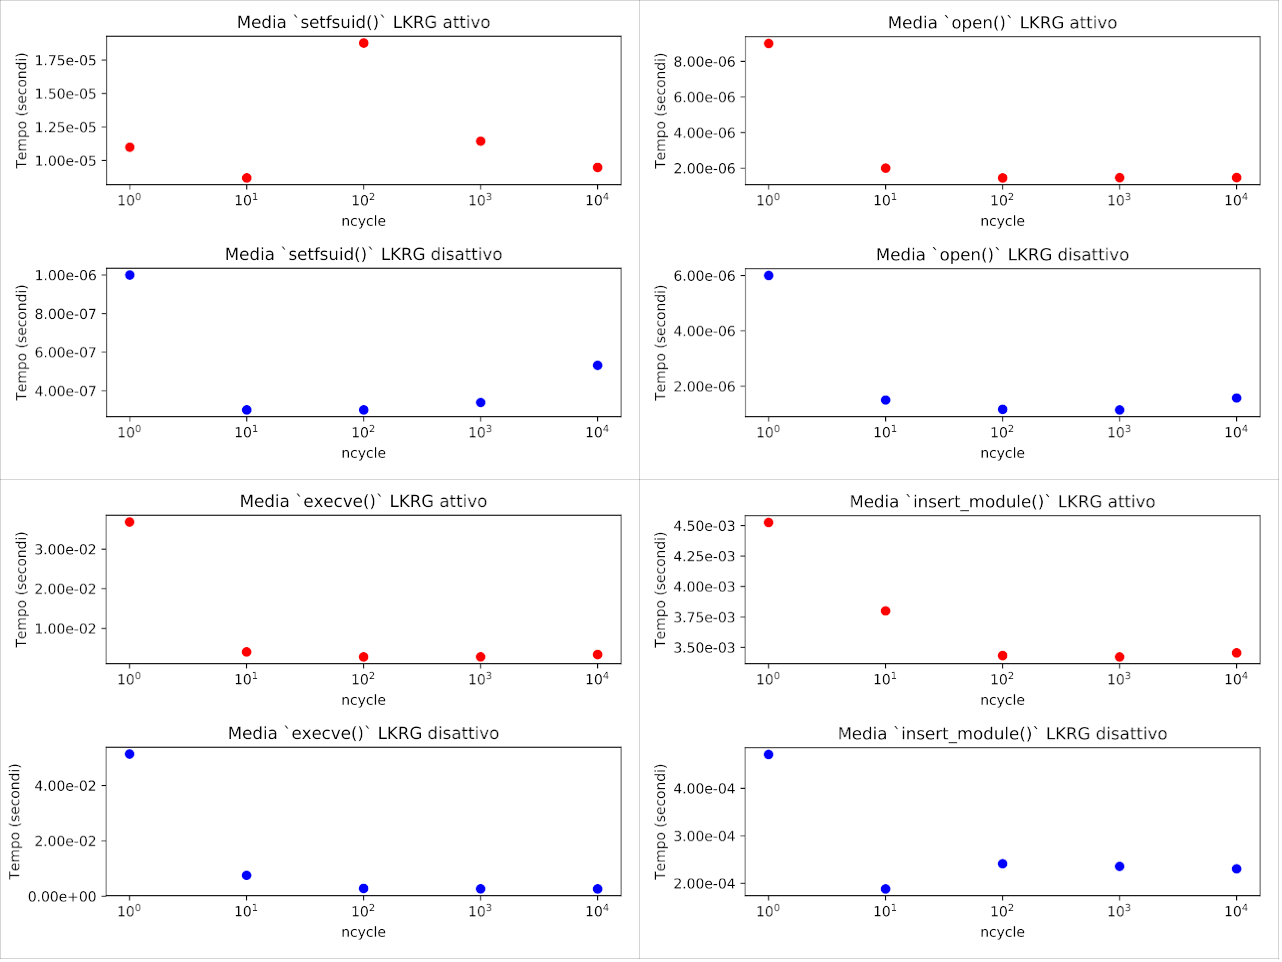
\includegraphics[scale=1.3]{Figures/Debian/Mean3}
\caption[Media singole system call nei 5 benchmark parte 3 (Debian)]{Media singole system call nei 5 benchmark parte 3 (Debian).}
\label{fig:mean3DebianFig}
\end{figure}

\begin{figure}[!htbp]
\centering
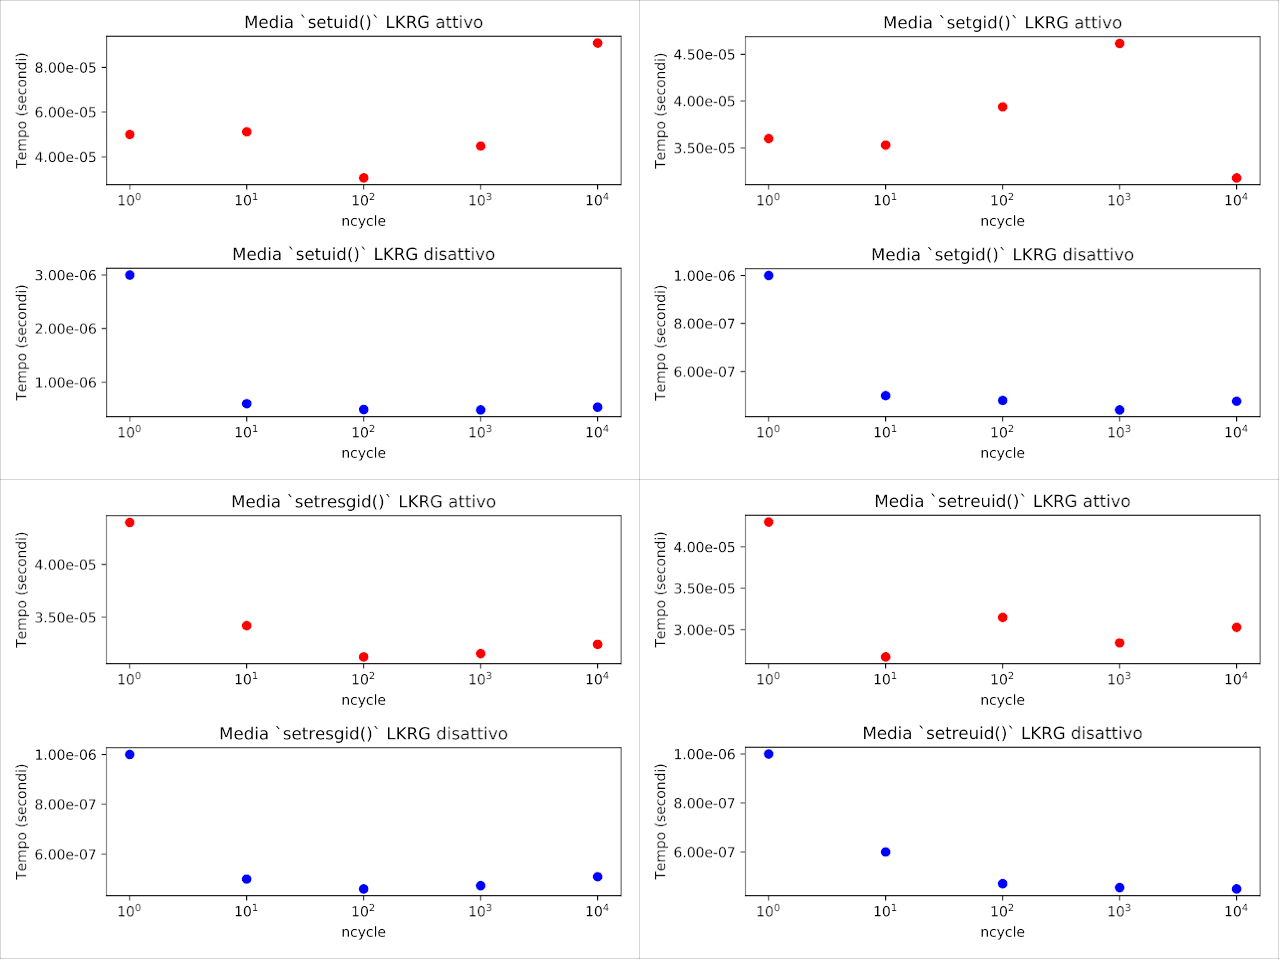
\includegraphics[scale=1.3]{Figures/Debian/Mean4}
\caption[Media singole system call nei 5 benchmark parte 4 (Debian)]{Media singole system call nei 5 benchmark parte 4 (Debian).}
\label{fig:mean4DebianFig}
\end{figure}

Nei grafici rappresentati in queste quattro figure è immediato notare l'andamento esponenziale dei tempi delle singole chiamate di sistema quando il modulo non è attivo. A differenza dei tempi misurati in Ubuntu, questi valori sono più stabili e la curva esponenziale che formano è ancora più evidente e precisa. I valori misurati con LKRG caricato nel kernel rimangono invece abbastanza instabili per la maggior parte delle system call, mentre per altre come la \emph{open()} mantengono un andamento esponenziale simile a quelli misurati in assenza del modulo, sebbene siano leggermente più elevati.

%----------------------------------------------------------------------------------------
%	MINT TESTS
%----------------------------------------------------------------------------------------
\section{Test in Mint}

L'ultimo sistema da testare, nonchè uno tra i più conosciuti ed utilizzati, è Linux Mint. I test hanno rilevato un comportamento differente del sistema, i cui risultati talvolta convergono a quelli ottenuti in Ubuntu, mentre per certe system call sono intermedi tra quelli di Ubuntu e Debian.

In \autoref{fig:setxMintFig} sono riportati i grafici ottenuti mediante la solita esecuzione di SysBench con ncycle=1, come per le altre valutazioni.

Il primo commento in merito ai grafici riguarda il comportamento della funzione \emph{setgid()}: il tempo d'esecuzione di tale funzione, escluso qualche test eccezionale, non varia in maniera clamorosa tra la misurazione con LKRG e senza. Inoltre, anche la \emph{setuid()} e molte altre di queste funzioni presentano risultati più analoghi, sebbene leggermente differenti ma di un fattore irrilevante, a quelli ottenuti in Debian rispetto a quelli in Ubuntu, nei quali vi era più di un test fuori dalla media.
Per altre system call come la \emph{setregid()} e la \emph{setfsuid()} si può affermare l'opposto. La distribuzione dei grafici risulta essere abbastanza chiara come negli altri sistemi, facilitando la lettura e indicando in maniera chiara l'overhead causato da LKRG; si osservi che a seconda della system call il fattore di differenza tra i tempi d'esecuzione è circa 1.5, 3, 10 o 100.

\begin{table}[!htbp]
\centering
\begin{tabular}{|c|c|c|c|c|}
\hline
\textbf{SystemCall} & \bm{$\overline{x}$} \textbf{loaded} & \bm{$\overline{x}$} \textbf{unloaded} & \bm{$\sigma$} \textbf{loaded} & \bm{$\sigma$} \textbf{unloaded}\\
\hline
setuid() & 3.862e-05 & 2.060e-06 & 1.062e-05 & 4.200e-07 \\
\hline
setgid() & 4.658e-04 & 3.863e-04 & 1.436e-04 & 5.517e-05 \\
\hline
setresuid() & 3.212e-05 & 1.380e-06 & 4.325e-06 & 4.854e-07 \\
\hline
setresgid() & 3.843e-03 & 1.052e-03 & 3.305e-04 & 8.837e-05 \\
\hline
setreuid() & 2.392e-05 & 1.120e-06 & 1.707e-06 & 1.608e-06 \\
\hline
setregid() & 4.811e-03 & 1.473e-03 & 3.432e-04 & 1.055e-04 \\
\hline
setfsuid() & 2.276e-05 & 6.800e-07 & 1.871e-06 & 4.665e-07 \\
\hline
setfsgid() & 2.278e-05 & 4.800e-07 & 3.402e-06 & 4.996e-07 \\
\hline
\end{tabular}
\caption{Dati benchmark funzioni \emph{setX()} con ncycle=1 (Mint)}
\label{table:setxMintData}
\end{table}

Nella tabella \autoref{table:setxMintData} si noti come la deviazione standard dei valori quando il modulo è attivo sia sempre maggiore rispetto a quella calcolata in sua assenza. Ugualmente, anche la media delle singole chiamate è sempre minore, talvolta persino 100 volte più piccola se prendiamo in considerazione la \emph{setfsuid()} e la \emph{setfsgid()}. 

\clearpage

\begin{figure}[!ht]
\centering
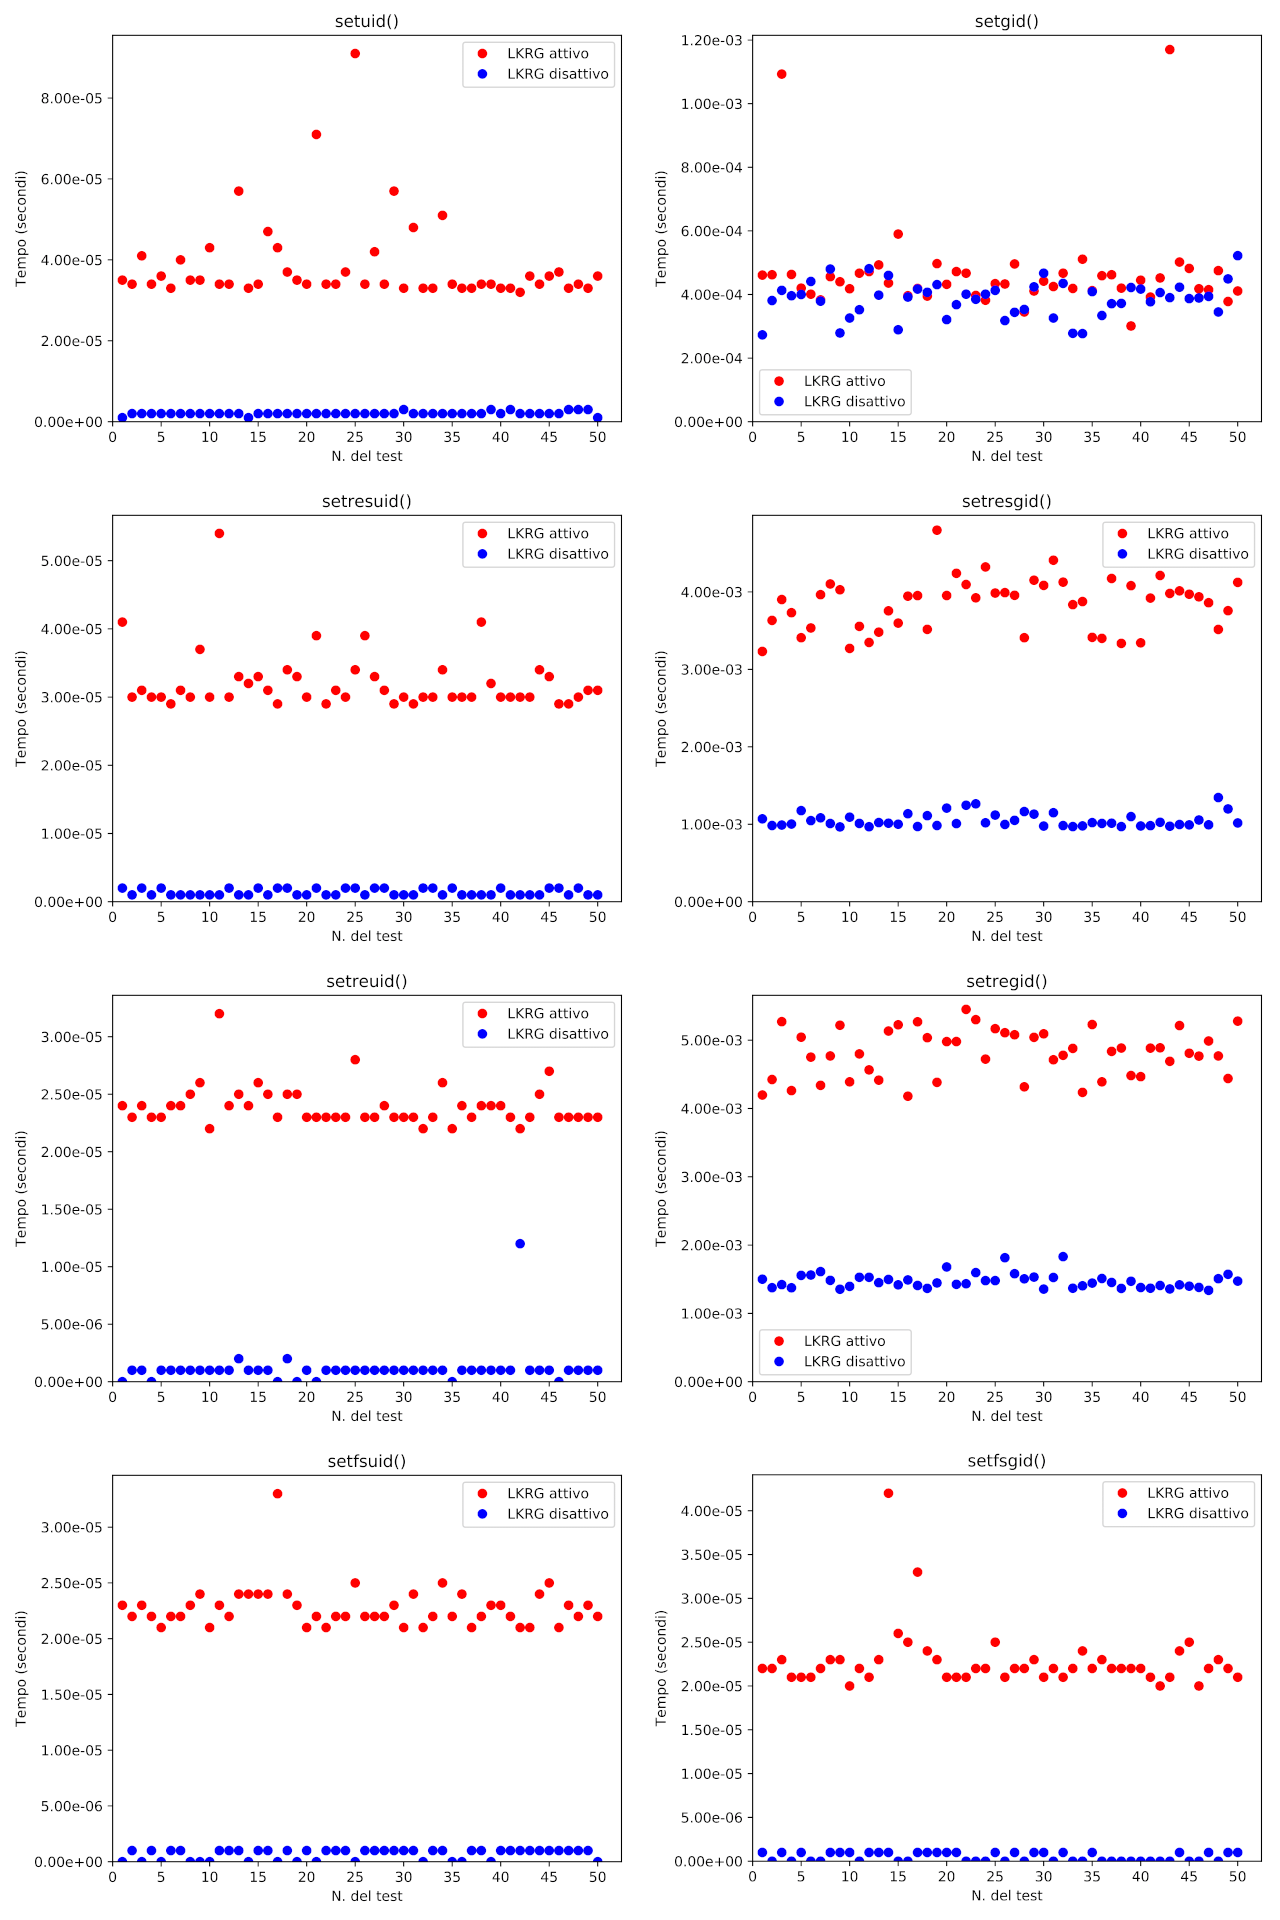
\includegraphics[scale=1.35]{Figures/Mint/SingleSet}
\caption[Benchmark funzioni \emph{setX} con ncycle=1 (Mint)]{Benchmark funzioni \emph{setX} con ncycle=1 (Mint).}
\label{fig:setxMintFig}
\end{figure}

Si può dedurre che il sovraccarico di istruzioni aggiunte da LKRG non sia trascurabile se ci atteniamo a considerare i risultati all'interno del loro ordine di grandezza. Infatti, la maggior parte delle funzionalità nella tabella hanno dei tempi molto differenti.


I risultati delle system call raffigurate in figura \autoref{fig:othersMintFig} si avvicinano maggiormente a quelli ottenuti in Ubuntu rispetto a Debian, ad esclusione della \emph{insert\_module()}; quest'ultima ha un comportamento interessante anche in Mint, dato che i valori massimi sono registrati quando nel sistema non vi è LKRG. Per quanto riguarda le altre funzionalità, esse hanno un andamento stabile come si può osservare dai grafici: i valori ottenuti in assenza del modulo sono abbastanza omogenei tra loro con poche misurazioni isolate, e lo stesso vale per gli altri.

\begin{figure}[!ht]
\centering
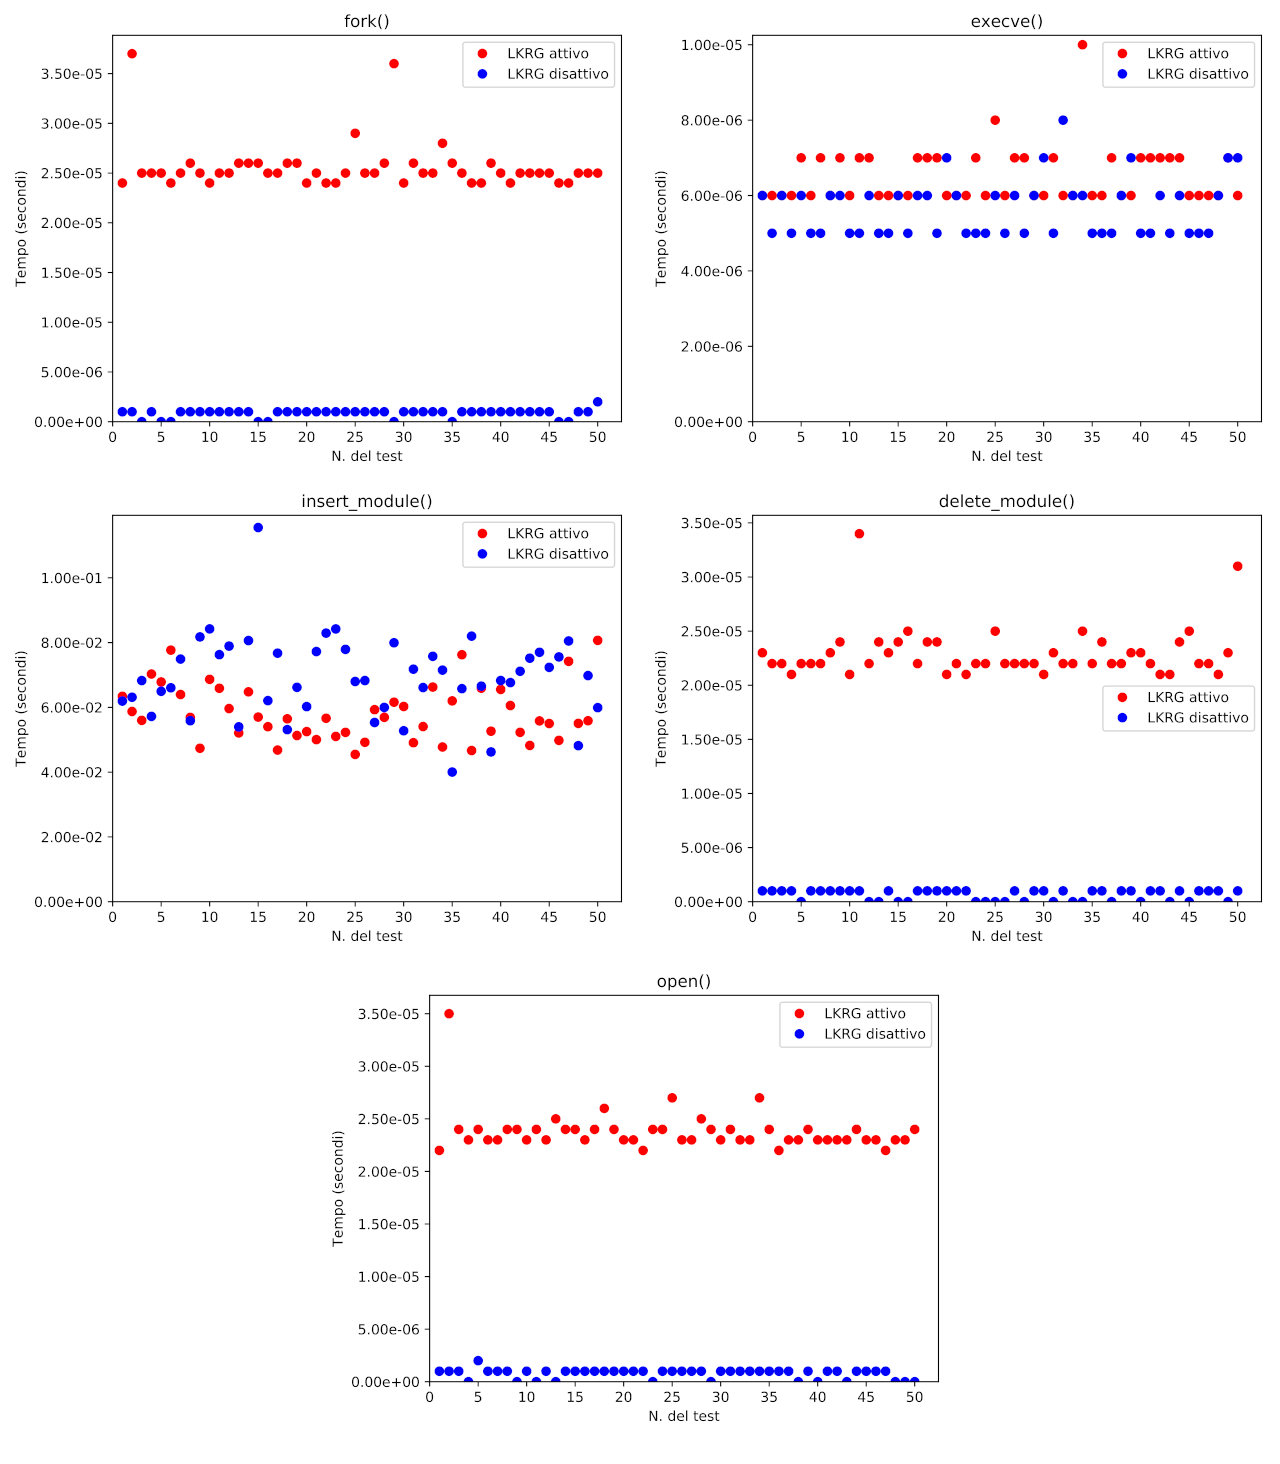
\includegraphics[scale=1.35]{Figures/Mint/SingleOthers}
\caption[Benchmark restanti funzioni con ncycle=1 (Mint)]{Benchmark restanti funzioni con ncycle=1 (Mint).}
\label{fig:othersMintFig}
\end{figure}

\begin{table}[!htbp]
\centering
\begin{tabular}{|c|c|c|c|c|}
\hline
\textbf{SystemCall} & \bm{$\overline{x}$} \textbf{loaded} & \bm{$\overline{x}$} \textbf{unloaded} & \bm{$\sigma$} \textbf{loaded} & \bm{$\sigma$} \textbf{unloaded}\\
\hline
open() & 2.380e-05 & 7.800e-07 & 1.908e-06 & 4.600e-07 \\
\hline
fork() & 2.556e-05 & 8.400e-07 & 2.434e-06 & 4.176e-07 \\
\hline
execve() & 6.500e-06 & 5.640e-06 & 7.280e-07 & 7.419e-07 \\
\hline
insert\_module() & 5.817e-02 & 6.920e-02 & 8.481e-03 & 1.234e-02 \\
\hline
delete\_module() & 2.292e-05 & 6.400e-07 & 2.288e-06 & 4.800e-07 \\
\hline
\end{tabular}
\caption{Dati benchmark restanti funzioni con ncycle=1 (Mint)}
\label{table:othersMintData}
\end{table}

I dati nella \autoref{table:othersMintData} confermano quanto appena detto: il valore medio d'esecuzione della singola \emph{insert\_module()} è effettivamente inferiore quando il modulo è caricato nel kernel, mentre tutti gli altri sono superiori in sua presenza. La funzione \emph{execve()} mantiene circa lo stesso tempo per le due tipologie d'esecuzione, e le deviazioni standard differiscono per un fattore piccolissimo di $2e^{-8}$. I tempi relativi alle altre system call invece variano come nei test relativi agli altri sistemi, passando da valori di ordine $10^{-7}$ a ordine $10^{-5}$, aumentando di conseguenza anche la deviazione standard. Infine nella \emph{delete\_module()} sono stati registrati molti valori pari a 0 senza LKRG, mentre, in presenza del modulo, il tempo minimo registrato è $2x10^{-5}$, un valore comunque molto più elevato della media.
Riguardo la \emph{execve()} si può affermare che il tempo d'esecuzione non sia influenzato in maniera evidente, assumendo valori poco discostanti tra loro come nei precedenti test.
\\\par

Concludiamo l'analisi presentando l'ultimo test di SysBench nei grafici in \autoref{fig:totMintFig} con i relativi dati nella \autoref{table:totMintData}, in cui ncycle assume valori esponenziali per dedurre se anche in questo sistema sono apportate alcune ottimizzazioni.

\begin{table}[!htbp]
\centering
\begin{tabular}{|c|c|c|c|c|}
\hline
\textbf{SystemCall} & \bm{$\overline{x}$} \textbf{loaded} & \bm{$\overline{x}$} \textbf{unloaded} & \bm{$\sigma$} \textbf{loaded} & \bm{$\sigma$} \textbf{unloaded}\\
\hline
setuid() & 2.797e-05 & 8.407e-07 & 8.672e-06 & 5.848e-07 \\
\hline
setgid() & 2.303e-05 & 5.871e-07 & 2.276e-06 & 2.066e-07 \\
\hline
setresuid() & 2.154e-05 & 6.193e-07 & 1.564e-06 & 1.922e-07 \\
\hline
setresgid() & 2.403e-05 & 6.368e-07 & 3.550e-06 & 1.966e-07 \\
\hline
setreuid() & 2.211e-05 & 6.051e-07 & 1.311e-06 & 2.040e-07 \\
\hline
setregid() & 2.108e-05 & 5.922e-07 & 9.071e-07 & 2.245e-07 \\
\hline
setfsuid() & 2.045e-05 & 3.754e-07 & 9.822e-07 & 1.889e-07 \\
\hline
setfsgid() & 2.128e-05 & 5.454e-07 & 1.969e-06 & 2.304e-07 \\
\hline
open() & 2.758e-06 & 2.278e-06 & 1.629e-06 & 1.382e-06 \\
\hline
fork() & 4.135e-04 & 3.156e-04 & 8.257e-05 & 7.042e-05 \\
\hline
execve() & 1.420e-02 & 1.468e-02 & 2.009e-02 & 2.152e-02 \\
\hline
insert\_module() & 4.086e-03 & 4.353e-04 & 3.770e-04 & 5.066e-04 \\
\hline
delete\_module() & 3.488e-03 & 2.788e-04 & 9.300e-05 & 3.561e-04 \\
\hline
\end{tabular}
\caption{Dati benchmark con ncycle=1, 10, 100, 1000, 10000 (Mint)}
\label{table:totMintData}
\end{table}

Il primo dettaglio da commentare è relativo alla funzione \emph{setfsuid()} nel grafico con ncycle=1, il cui campionamento ha rilevato un tempo d'esecuzione pari a 0 in assenza di LKRG, diversamente da quanto visto fino ad ora negli altri sistemi. Come è stato possibile osservare nel grafico in \autoref{fig:setxMintFig} l'esecuzione di tale funzione è spesso nulla, per questo motivo nel grafico in \autoref{fig:totMintFig} il tempo è pari a 0. Generalmente si può affermare che le funzionalità con il rapporto $\frac{Tattivo}{Tdisattivo}$ massimo sono le \emph{setX()} com'era risultato negli altri sistemi.

\begin{figure}[!ht]
\centering
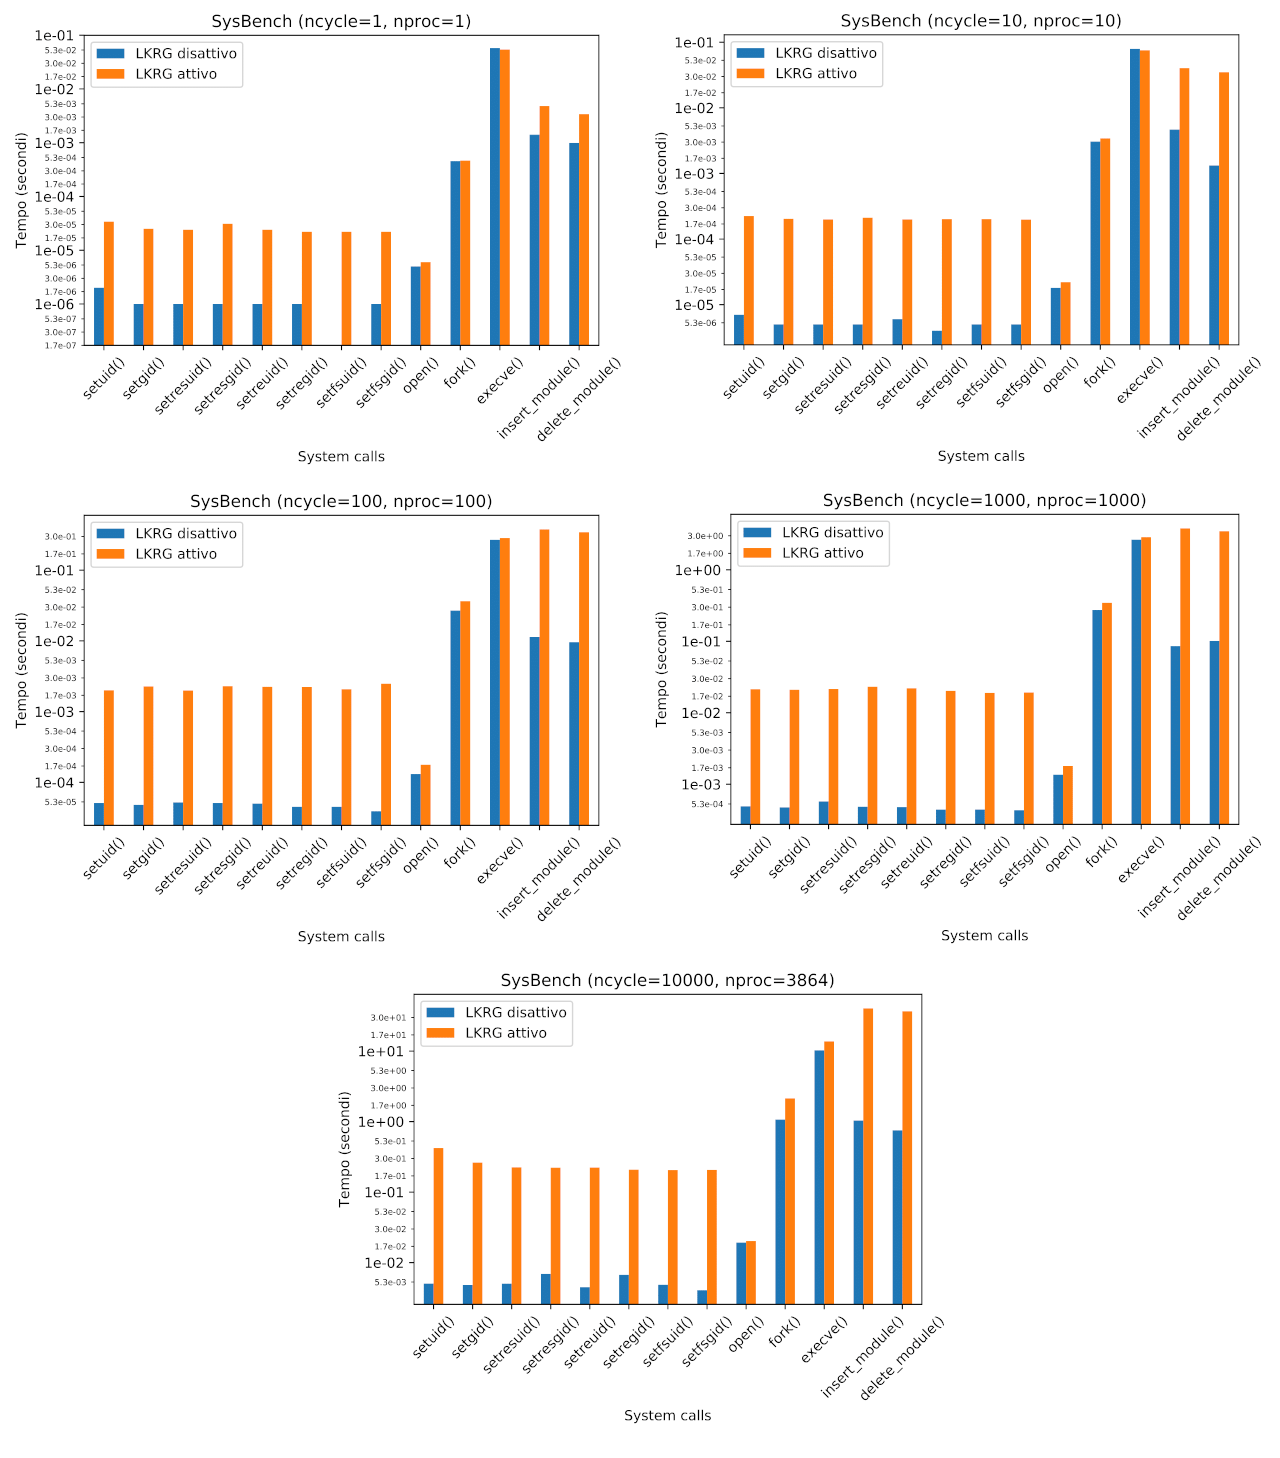
\includegraphics[scale=1.3]{Figures/Mint/Total}
\caption[Benchmark tempo totale (Mint)]{Benchmark tempo totale (Mint).}
\label{fig:totMintFig}
\end{figure}

La \emph{open()}, \emph{execve()} e la \emph{fork()} risultano ancora una volta essere le system call meno influenzate, i cui tempi d'esecuzione variano talmente poco che durante il test è quasi impercettibile la differenza (un paio di secondi in più per la execve quando il modulo è attivo e ncycle=10000). I tempi in relazione al loro ordine di grandezza ottenuti in seguito al test della \emph{insert\_module()} e \emph{delete\_module()} sono i più elevati, per cui la differenza lanciando un programma che esegue tali funzionalità diventa tanto più evidente quanto incrementa il numero di volte che vengono invocate: ad esempio considerando la prima delle due, la quale presenta una differenza pari a $3x10^{-3}$ tra le due esecuzioni e lanciando il test in cui tale system call viene invocata 10000 volte, il tempo d'esecuzione, non considerando le ottimizzazioni, aumenterebbe di $3x10^{1}$ volte, ovvero 30 secondi.

Nella \autoref{table:totMintData} sono riportati i dati di tutte le system call relativi a quest'ultimo test. Si osservi nuovamente che questi dati si discostano parecchio da quelli contenuti nella \autoref{table:setxMintData} e \autoref{table:othersMintData}, come era già successo nei casi precedenti. Vi è persino una differenza di $10^{2}$ tra il valore medio della singola esecuzione di \emph{insert\_module()} presentato in questa tabella e quello in \autoref{table:othersMintData}. Perciò è corretto assumere che vi sia stato un intervento di ottimizzazione, come si può osservare nei grafici sottostanti.

Anche in questo sistema è risultato che il tempo medio della singola system call ad esclusione della \emph{setfsuid()} diminuisce in base al numero di volte che viene richiamata. Nei grafici successivi è possibile osservare come il tempo d'esecuzione delle chiamate quando LKRG non è caricato risulta essere massimo nel test con ncycle=1, mentre raggiunge il minimo valore registrato nel test con ncycle=10000. In presenza del modulo, il tempo di tali funzionalità è molto variabile, talvolta esponenziale come nel grafico della \emph{execve()} in \autoref{fig:mean3MintFig}, mentre altre volte raggiunge dei picchi di massimo e minimo per poi variare nuovamente (si veda la \emph{fork()} o la \emph{setfsuid()}).

Si ricorda che per questi ultimi grafici è stata utilizzata una scala logaritmica per l'asse delle x, in modo tale da rappresentare i valori esponenziali assunti da ncycle.

\begin{figure}[!htbp]
\centering
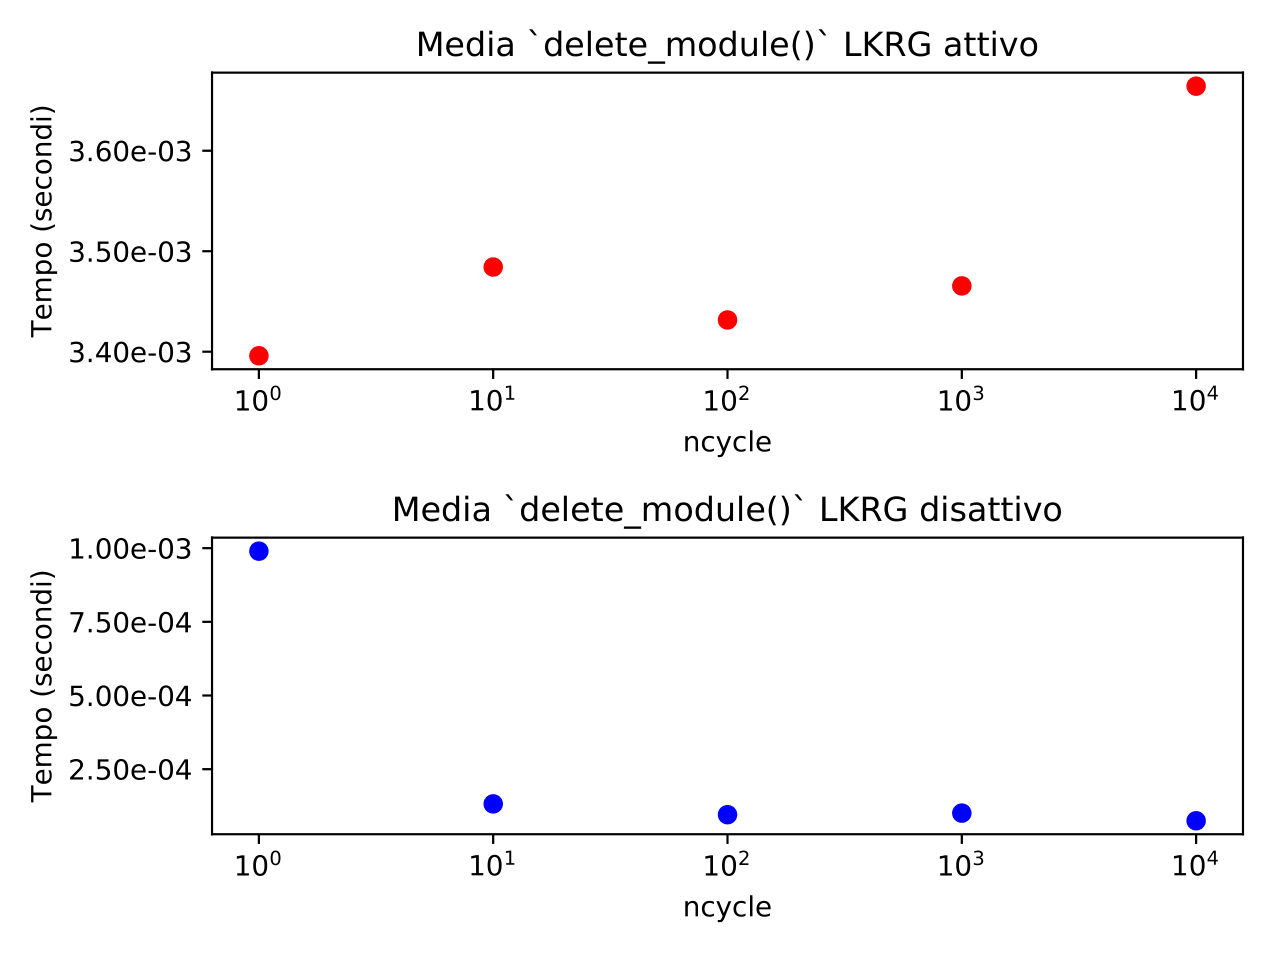
\includegraphics[scale=0.25]{Figures/Mint/Mean1}
\caption[Media singole system call nei 5 benchmark parte 1 (Mint)]{Media singole system call nei 5 benchmark parte 1 (Mint).}
\label{fig:mean1MintFig}
\end{figure}

\begin{figure}[!htbp]
\centering
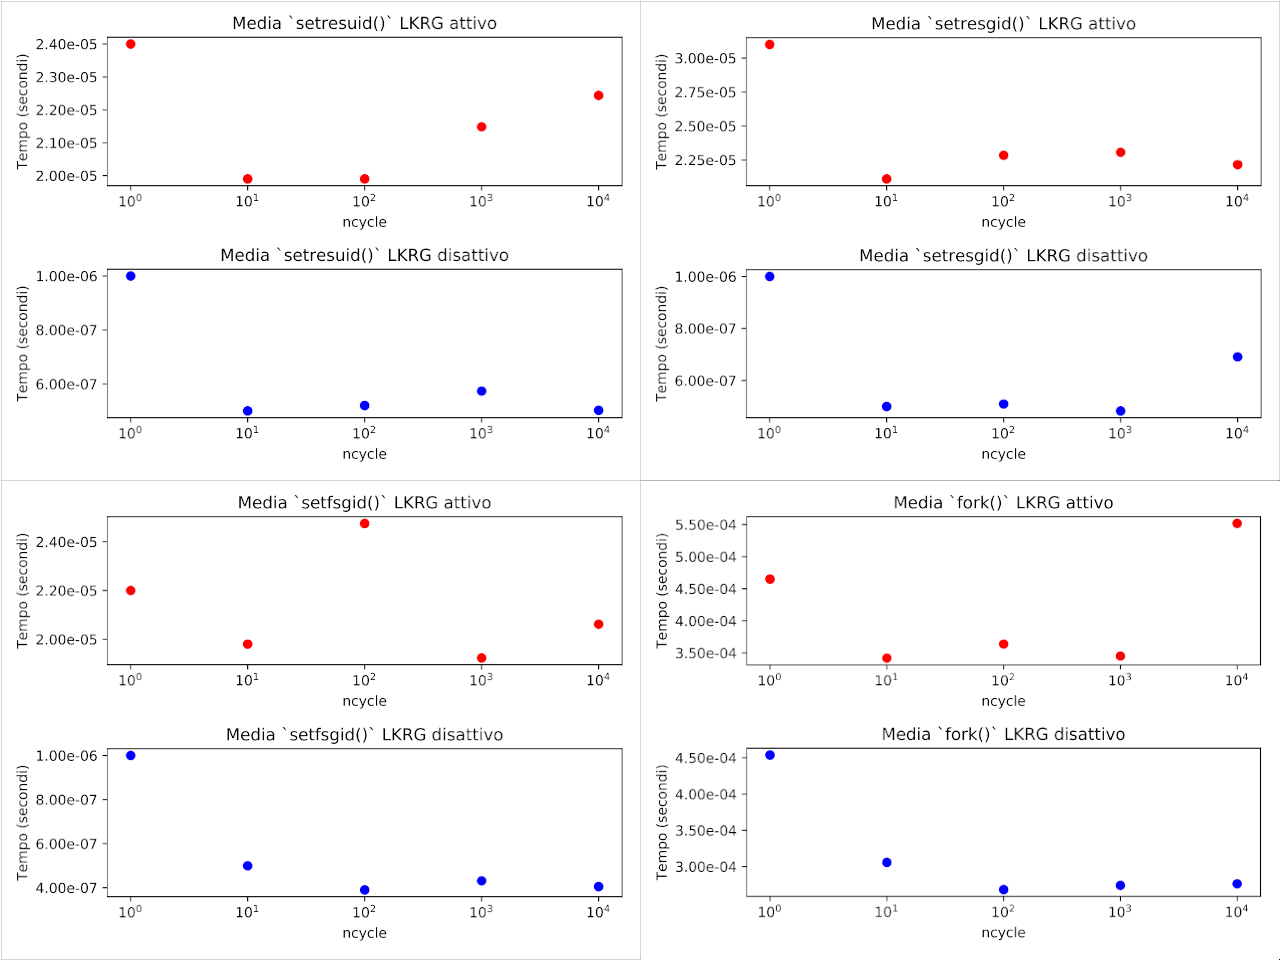
\includegraphics[scale=1.35]{Figures/Mint/Mean2}
\caption[Media singole system call nei 5 benchmark parte 2 (Mint)]{Media singole system call nei 5 benchmark parte 2 (Mint).}
\label{fig:mean2MintFig}
\end{figure}

\begin{figure}[!htbp]
\centering
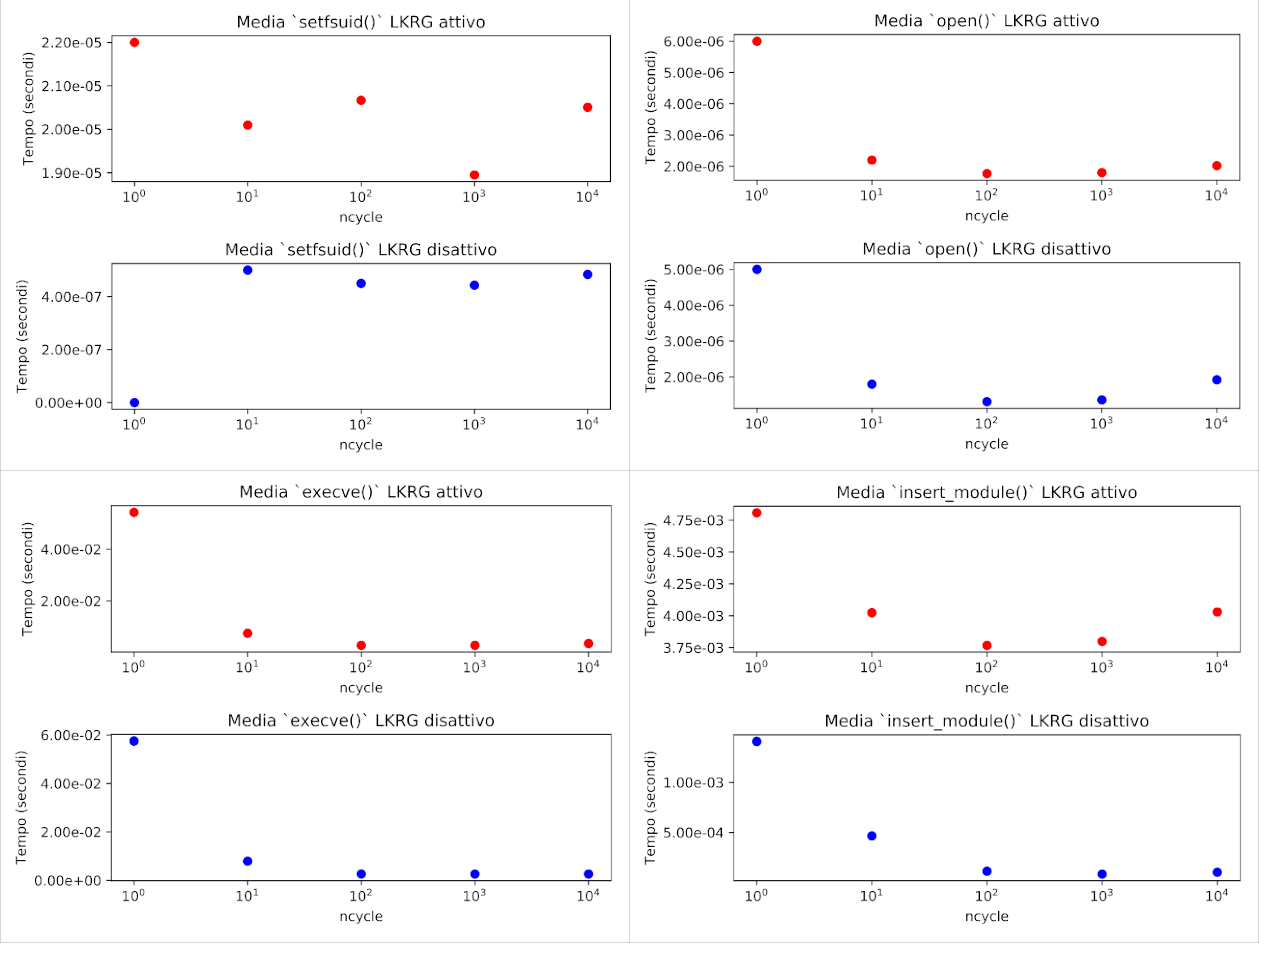
\includegraphics[scale=1.35]{Figures/Mint/Mean3}
\caption[Media singole system call nei 5 benchmark parte 3 (Mint)]{Media singole system call nei 5 benchmark parte 3 (Mint).}
\label{fig:mean3MintFig}
\end{figure}

\begin{figure}[!htbp]
\centering
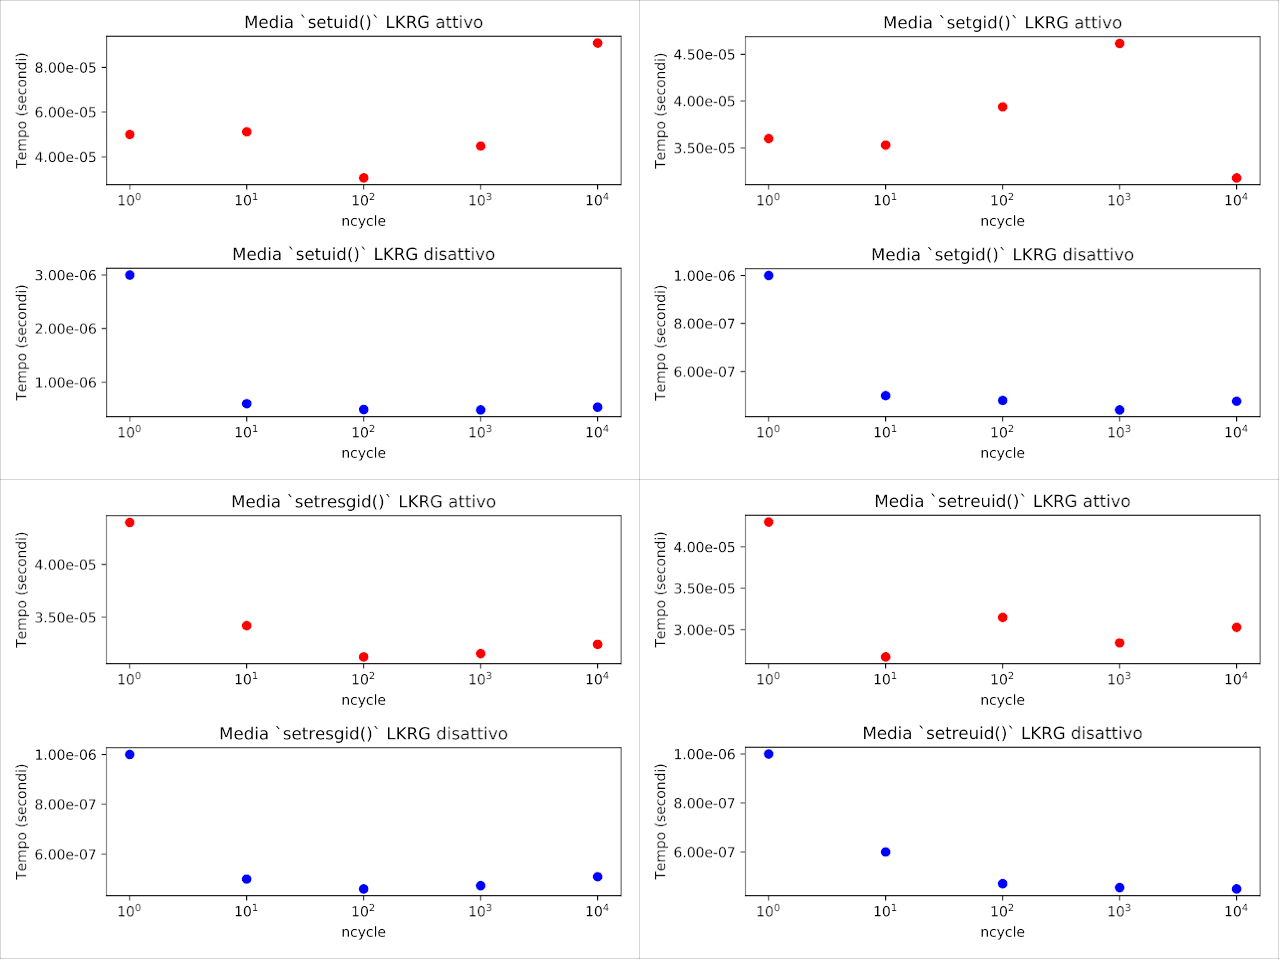
\includegraphics[scale=1.35]{Figures/Debian/Mean4}
\caption[Media singole system call nei 5 benchmark parte 4 (Mint)]{Media singole system call nei 5 benchmark parte 4 (Mint).}
\label{fig:mean4MintFig}
\end{figure}

%----------------------------------------------------------------------------------------
%	COMPARISON
%----------------------------------------------------------------------------------------
\section{I tre sistemi a confronto}

Nel corso della trattazione dei test nei vari sistemi sono già state anticipate alcune somiglianze e differenze dei risultati. In questa sezione conclusiva l'attenzione è rivolta all'aumento percentuale del tempo d'esecuzione delle system call in seguito al caricamento di \emph{Linux Kernel Runtime Guardian}, commentando appropriatamente i valori ottenuti. Per ottenere in formule matematiche il tempo misurato con LKRG presente, bisogna attenersi alla legge:\\
$T_f = T_i + x\%T_i => T_f = T_i * (1 + x\%)$

Ad esempio se una chiamata presenta un aumento pari al 100\%, il tempo finale è $T_f = T_i * (1 + 100\%) = T_i * 2 = 2T_i$, ovvero il doppio.

\begin{table}[!htbp]
\centering
\begin{tabular}{|c|c|c|c|c|}
\hline
\textbf{SystemCall} & \bm{$\Delta$}\textbf{ Ubuntu (\%)} & \bm{$\Delta$}\textbf{ Debian (\%)} & \bm{$\Delta$}\textbf{ Mint (\%)} \\
\hline
setuid() & 2332 & 2193 & 1875 \\
\hline
setgid() & 213 & 102 & 121 \\
\hline
setresuid() & 3659 & 735 & 2328 \\
\hline
setresgid() & 296 & 1597 & 365 \\
\hline
setreuid() & 3144 & 1478 & 2136 \\
\hline
setregid() & 283 & 884 & 327 \\
\hline
setfsuid() & 3406 & 1519 & 3347 \\
\hline
setfsgid() & 3824 & 1861 & 4746 \\
\hline
open() & 3089 & 1978 & 3051 \\
\hline
fork() & 2792 & 1906 & 3043 \\
\hline
execve() & 123 & 143 & 115 \\
\hline
insert\_module() & 137 & 75 & 84 \\
\hline
delete\_module() & 3432 & 1411 & 3581 \\
\hline
\hline
Media & 2056 & 1222 & 1932 \\
\hline
\end{tabular}
\caption{Aumento percentuale tempo d'esecuzione nei 3 sistemi}
\label{table:compareData}
\end{table}

Dalla \autoref{table:compareData} si evince che le system call minormente influenzate dal modulo in tutti i sistemi sono la \emph{setuid()}, \emph{setregid()}, \emph{execve()} e \emph{insert\_module()}, in quanto il tempo d'esecuzione a causa dei controlli d'integrità raddoppia o triplica al massimo. Al contrario, le rimanenti funzioni subiscono un aumento rilevante che varia dal 800\% per la \emph{setregid()} (corrispondente a 9 volte il tempo iniziale) ad un massimo di 4746 per la \emph{setfsgid()}, ovvero poco più di $48T_i$.

Questi elevati valori porterebbero a pensare che LKRG rallenti pesantemente il sistema nel quale è installato, portando sfortunatamente alla conclusione sbagliata. Quando si osservano delle percentuali bisogna sempre fare riferimento ai tempi di partenza e al loro ordine di grandezza: ad esempio, un aumento del 100\% in una chiamata che impiega 1 secondo ad essere soddisfatta è più rilevante di un aumento pari a 5000\% di una system call il cui tempo d'esecuzione è dell'ordine di $10^{-7}$. Per questi motivi, dopo aver analizzato tutti i grafici ed i tempi riportati in questo capitolo, è possibile farsi un'idea circa l'effettivo overhead del sistema, riferendosi ad un caso d'uso personale.

Dai grafici e dai dati è risultato che sicuramente in tutti e tre i sistemi LKRG effettua i controlli con tempi differenti, nonostante l'installazione ed l'esecuzione di SysBench fosse avvenuta nelle medesime condizioni. L'ultima riga della tabella riporta l'incremento percentuale medio delle system call in ogni sistema; si osservi come in base a questi valori il sistema al quale LKRG aggiunge maggiore overhead risulti essere Ubuntu, seguito da Mint ed infine Debian.

Dovendo prestare attenzione ad un possibile scenario reale, si pensi ad un server hostato in un sistema Ubuntu, dal quale in base ad alcune richieste dell'utente vengono lanciati i comandi \emph{execve()}, \emph{fork()} e \emph{open()}. Essendo i tre maggiormente utilizzati si vuole valutare se vale la pena o meno inserire LKRG nel server, per evitare che il tempo di risposta del server renda l'esperienza utente meno gradevole. Dall'analisi è risultato che l'aumento in percentuale delle funzioni è rispettivamente pari a 123\%, 2792\% e 3089\%. Per cui assumento come tempi per ogni singola chiamata i valori riportati nella tabella \autoref{table:othersUbuntuData}, ovvero $7.74x10^{-6}, 3.518x10^{-5}$ e $3.398x10^{-5}$ ed ipotizzando che per ogni utente vengono gestite singolarmente mille istanze delle seguenti operazioni (ncycle=1 ntimes=1000, esecuzione di SysBench tramite lo script), si ha che:\\\\
$TempoFinale_{execve} = 7.74x10^{-6} * (1 + 1.23) * 1000 = 0.01726$ secondi\\
$TempoFinale_{fork} = 3.518x10^{-5} * (1 + 27.92) * 1000 = 1.01741$ secondi\\
$TempoFinale_{open} = 3.398x10^{-5} * (1 + 30.89) * 1000 = 1.0836222$ secondi
\\\par

Nonostante questo scenario sia estremo, in quanto non accadrà mai di gestire 1000 di queste system call per un singolo utente, si ha che la richiesta verrà soddisfatta nei tempi riportati, i quali sono estremamente bassi. Si pensi infatti se l'esperienza utente è veramente influenzata da un ritardo di 1 secondo in una risposta; sono tempi molto piccoli, difficile da percepire se non effettuandone una valutazione con un programma come SysBench.